\documentclass[12pt,letterpaper]{article}

% ── Fonts & Layout ─────────────────────────────────────────────
\usepackage[margin=0.75in]{geometry}
\usepackage[T1]{fontenc}
\usepackage[utf8]{inputenc}
\usepackage{helvet}
\renewcommand{\familydefault}{\sfdefault}
\usepackage{microtype}
\usepackage{setspace}
\setstretch{1.45}

% ── Packages ──────────────────────────────────────────────────
\usepackage{enumitem}
\usepackage{tabularx}
\usepackage{booktabs}
\usepackage{graphicx}
\usepackage{float}
\usepackage{amsmath}
\usepackage{xcolor}
\usepackage{subcaption}
\usepackage{caption}
\usepackage{indentfirst}
\usepackage[hidelinks]{hyperref}

\graphicspath{{figures/}}
\captionsetup{font=small,labelfont=bf,skip=6pt}

\setlist[itemize]{leftmargin=1.5em,noitemsep,topsep=3pt}
\setlist[enumerate]{leftmargin=1.5em,noitemsep,topsep=3pt}

% ── Section formatting ───────────────────────────────────────
\usepackage{titlesec}
\titlespacing*{\section}{0pt}{10pt}{4pt}
\titlespacing*{\subsection}{0pt}{8pt}{3pt}

\begin{document}

% ═══ Compact Title Block (not a full page) ════════════════════
\begin{center}
\vspace*{-1cm}
{\Large\bfseries The Effect of Feedback Modality on Speed--Accuracy\\[2pt]Tradeoff in a Visual Target-Selection Task}\\[10pt]
{\normalsize MIE\,286 -- Probability \& Statistics \hfill Winter 2026 \hfill Team 51}\\[4pt]
{\normalsize Markiyan Konyk \quad Jessica Yi \quad Memo Ozdincer}\\[3pt]
{\small University of Toronto \hfill April 7, 2026}
\end{center}
\vspace{0.3cm}
\noindent\rule{\textwidth}{0.4pt}
\vspace{0.3cm}


% ═══ 1. INTRODUCTION ══════════════════════════════════════════
\section{Introduction}

This project centers around a browser-based target-clicking game, where $N = 41$ university students were asked to play it under two different feedback conditions: one where the screen border flashes a color after each click (visual), and one where a tone plays instead (auditory). Our investigation was guided by the question: does the type of sensory feedback change how people balance speed and accuracy?

Figure~\ref{fig:interface} shows the game's interface. A blue target appears at a random position on an 800$\times$500\,px canvas; the participant clicks the blue dot as quickly as they can with precision. In the visual condition, the border glows gold (fast hit), green (slow hit), or red (miss). In the auditory condition, a high, medium, or low tone plays instead. Both convey the same three categories of information.

\begin{figure}[H]
\centering
\begin{subfigure}[t]{0.48\textwidth}
  \centering
  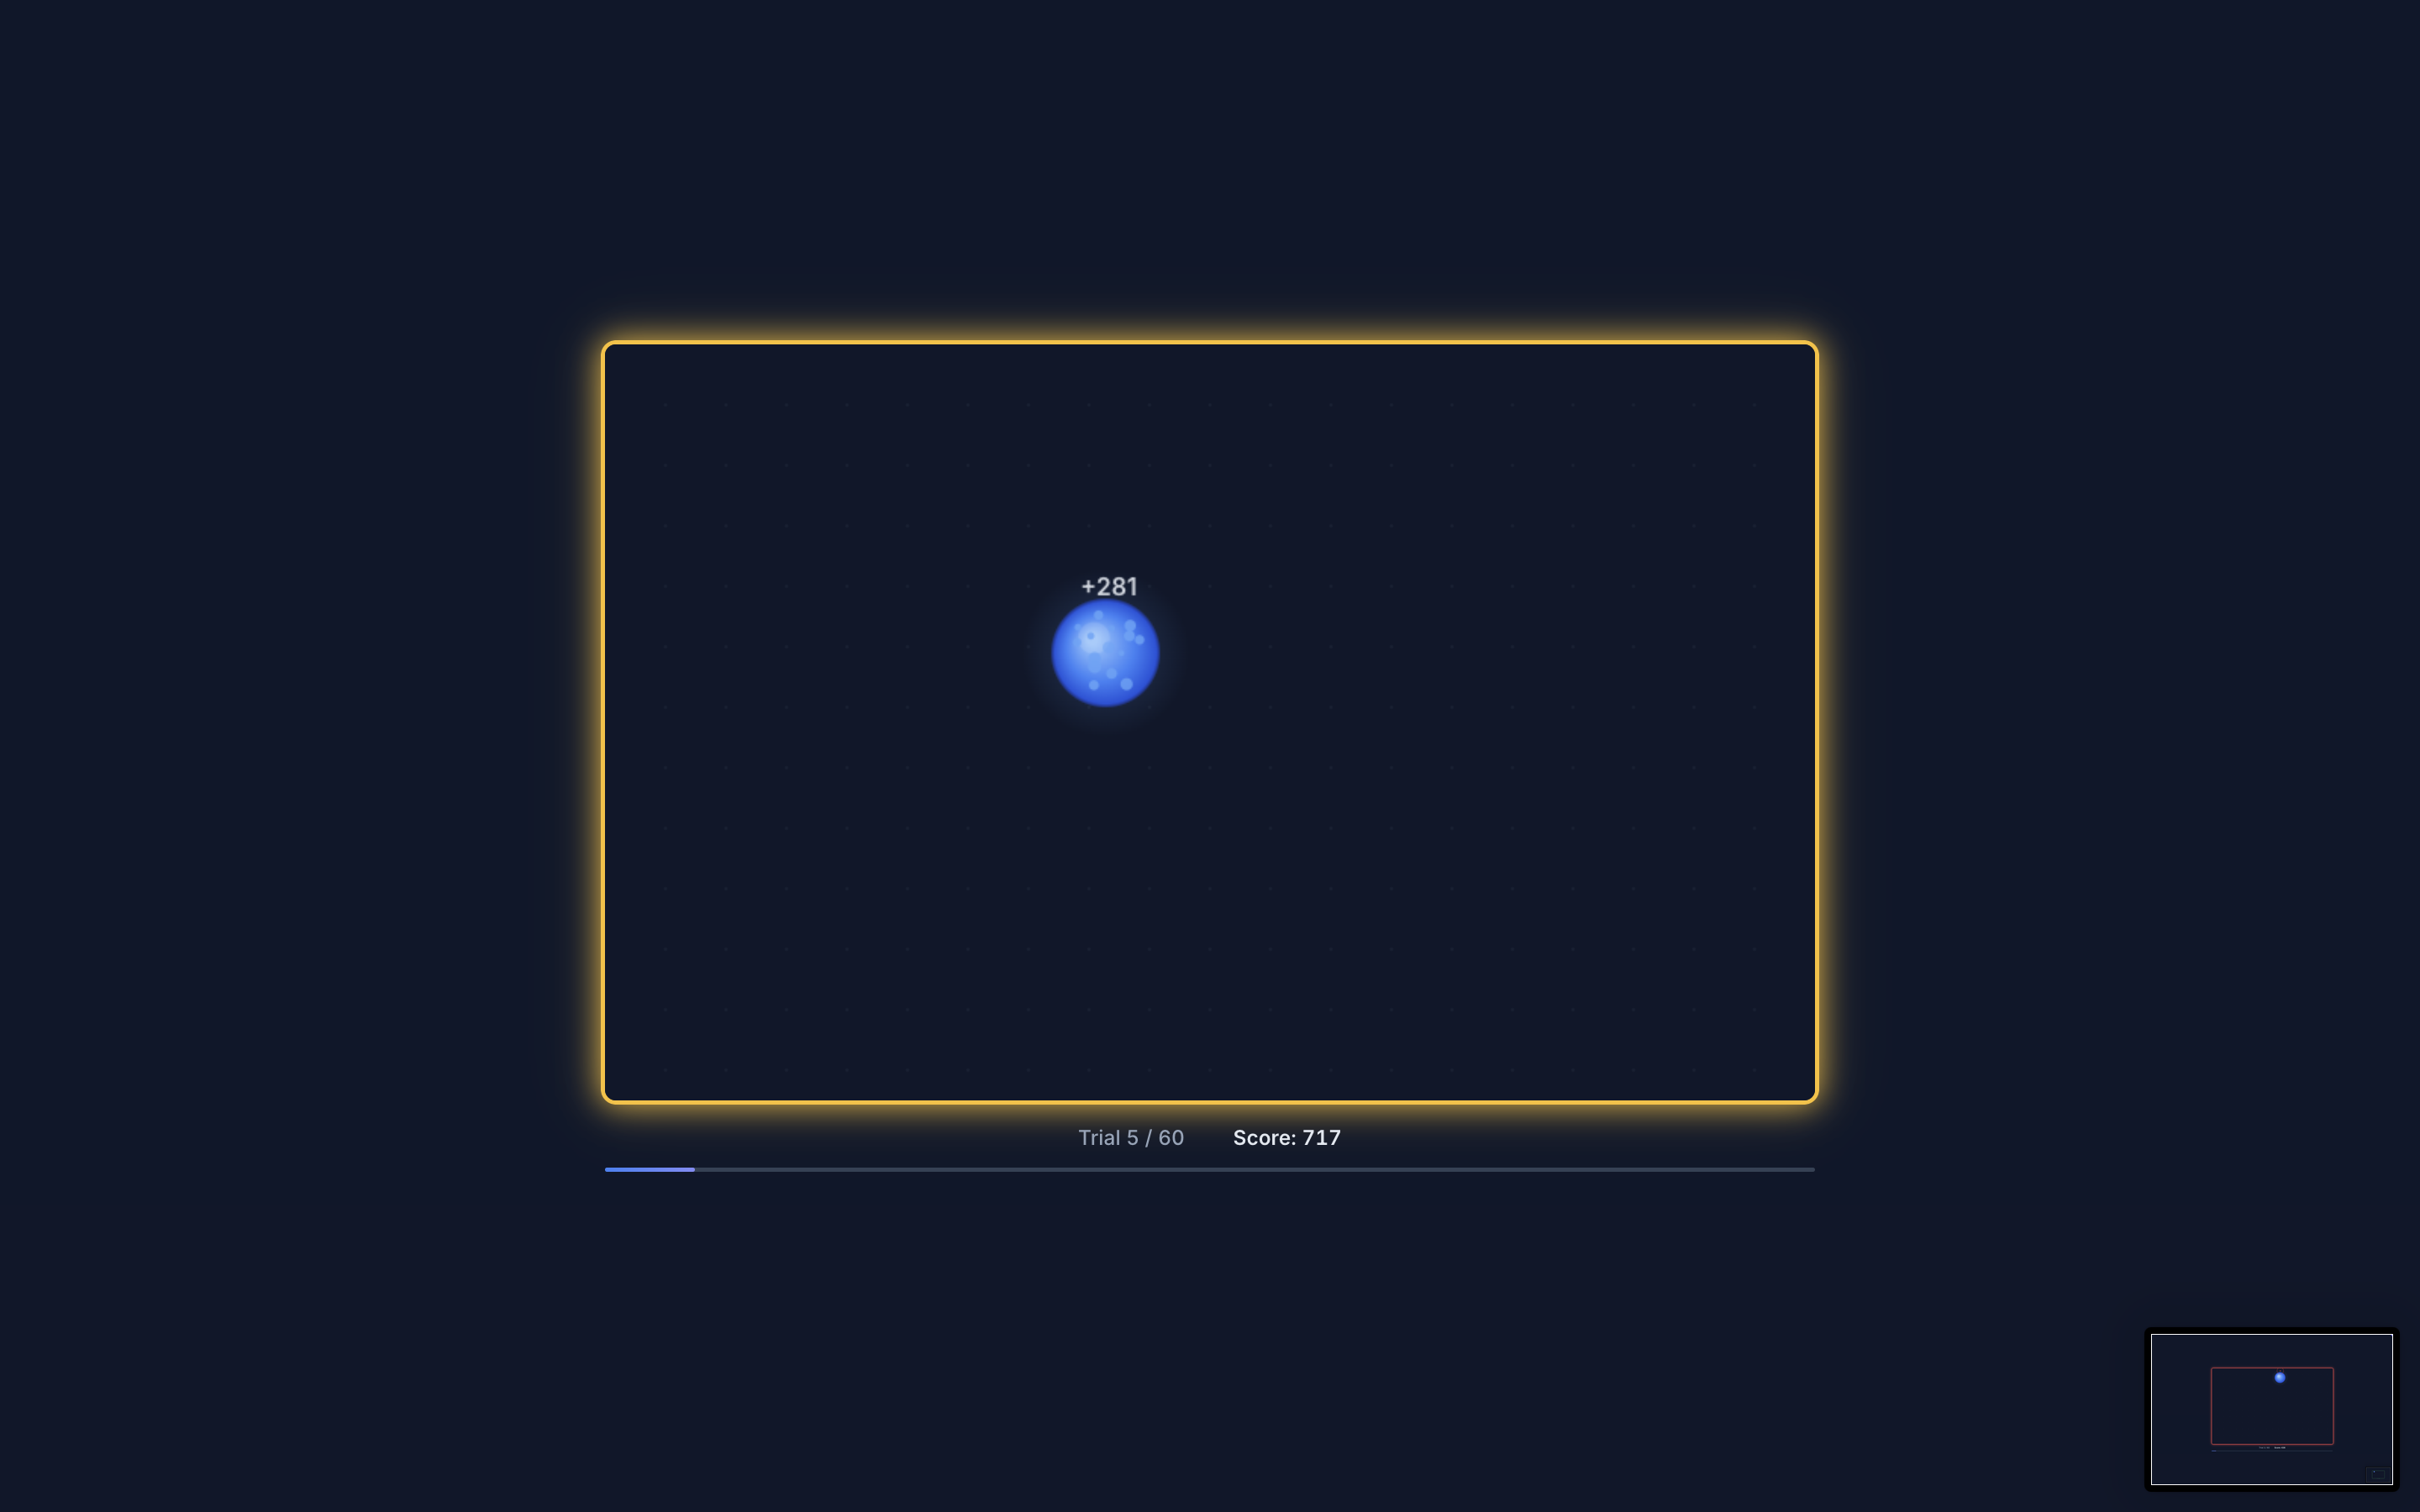
\includegraphics[width=\textwidth]{hit_gold_feedback_visual.png}
  \caption{Visual: gold glow = fast hit ($<$600\,ms)}
\end{subfigure}
\hfill
\begin{subfigure}[t]{0.48\textwidth}
  \centering
  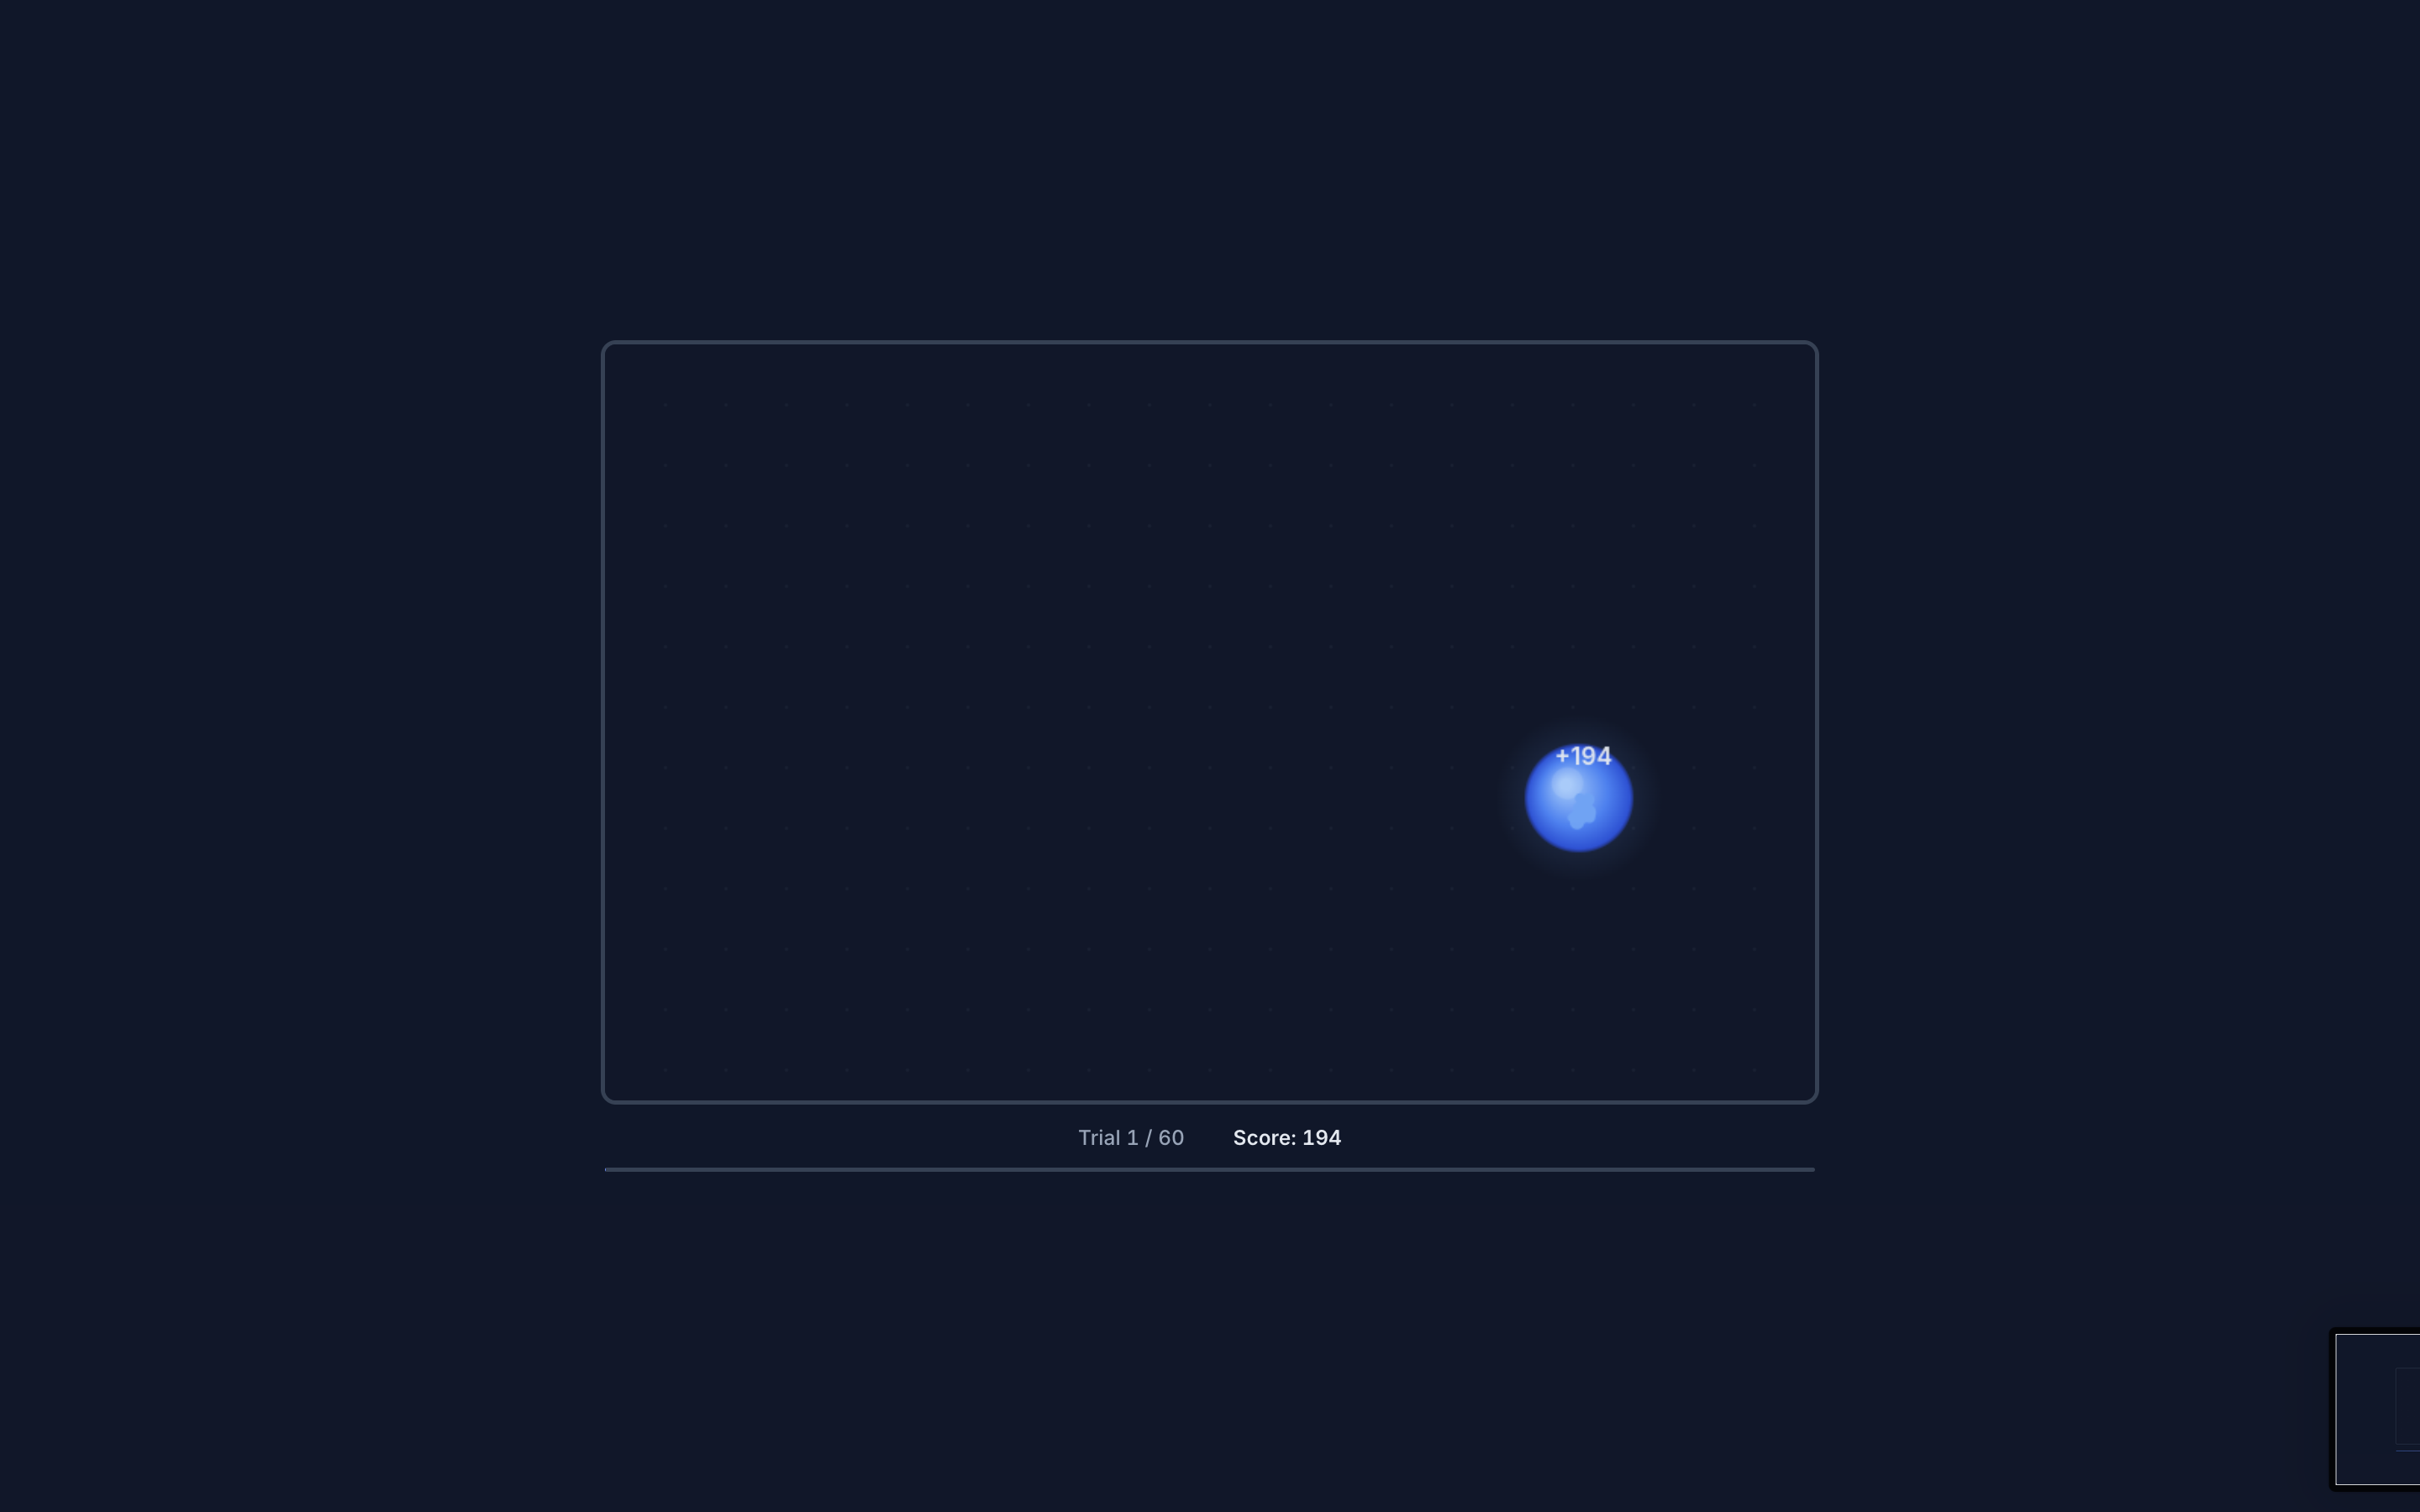
\includegraphics[width=\textwidth]{hit_on_audio_shows_no_visual_confimation.png}
  \caption{Auditory: no visual change, tone plays}
\end{subfigure}
\caption{The experiment interface in both conditions. The only difference is the feedback channel.}
\label{fig:interface}
\end{figure}

Wickens' Multiple Resource Theory~[1,\,2] predicts that a visual task paired with visual feedback should overload one attentional channel, suggesting that auditory feedback may be more effective for visual tasks. Cognitive Load Theory~[3] agrees: distributing information across modalities should reduce sensory burden. Thus, we expected that auditory feedback would enhance response speed and precision during the visual task.

Contrary to our original hypothesis, the collected data suggests that visual feedback made people \emph{faster}, not slower. The gold/green distinction created a visible speed target that participants actively chased; they were frustrated when they got green instead of gold. This motivational effect overrode the predicted interference. We tested three hypotheses:

\begin{enumerate}
  \item \textbf{H\textsubscript{1}:} Reaction time will differ between visual and auditory feedback.
  \item \textbf{H\textsubscript{2}:} The faster condition will have greater radial error (speed--accuracy tradeoff).
  \item \textbf{H\textsubscript{3}:} The speed--accuracy tradeoff \emph{structure} (slope of RT vs.\ error) will differ between conditions.
\end{enumerate}


% ═══ 2. BACKGROUND ════════════════════════════════════════════
\section{Background}

The speed--accuracy tradeoff (SAT) is a fundamental constraint: faster responses are generally less accurate. Heitz~[6] emphasizes that the SAT is not a single number but a \emph{function} whose shape can change across conditions. Fitts' Law~[4,\,5] characterizes motor pointing performance, but our task holds target size constant and randomizes position, so differences should reflect cognitive processing of feedback rather than pure motor constraints.

Prior work supports modality effects. Akamatsu et al.~[7] found auditory feedback reduced movement time in pointing tasks. Sigrist et al.~[8] reviewed evidence that auditory feedback supports motor learning through cross-modal facilitation. However, these studies examined mean performance; whether modality changes the SAT \emph{slope} remains open.


% ═══ 3. METHODS ═══════════════════════════════════════════════
\section{Methods}

\subsection{Participants}

A total of 72 participants (aged 18-23 years, all university students) took part in the study. Initially, the experiment used 30 trials per block, but preliminary analysis showed that 30 trials produced unstable per-participant statistics and the effects of interest (streak patterns, tilt cascades) were not visible. Thus, the number of trials was increased to 60 per block. Only participants who completed the full 60-trial protocol are included in the final analysis ($N = 41$); a full comparison of 30- vs.\ 60-trial cohorts is in Appendix~\ref{app:30v60}. Table~\ref{tab:sample} summarizes the final sample.

\begin{table}[H]
\centering
\caption{Participant demographics and covariates ($N = 41$).}
\label{tab:sample}
\begin{tabular}{llr}
\toprule
\textbf{Covariate} & \textbf{Level} & \textbf{$N$} \\
\midrule
\multirow{3}{*}{Input Device} & Mouse & 18 \\
 & Trackpad & 16 \\
 & Other & 7 \\[4pt]
\multirow{4}{*}{Gaming Frequency} & Never & 9 \\
 & Rarely & 13 \\
 & Weekly & 10 \\
 & Daily & 9 \\[4pt]
\multirow{2}{*}{Condition Order (randomized)} & Visual $\to$ Auditory & 17 \\
 & Auditory $\to$ Visual & 24 \\
\bottomrule
\end{tabular}
\end{table}

\subsection{Apparatus and Task}

The experiment interface was a browser-based application hosted on GitHub Pages. Targets (radius = 35\,px) appeared at random canvas positions and participants were instructed to click them as quickly and accurately as possible. Timing used the browser's \texttt{performance.now()} API (sub-millisecond precision). A 400\,ms inter-trial interval separated targets. Figure~\ref{fig:feedback_states} shows the three visual feedback states.

\begin{figure}[H]
\centering
\begin{subfigure}[t]{0.30\textwidth}
  \centering
  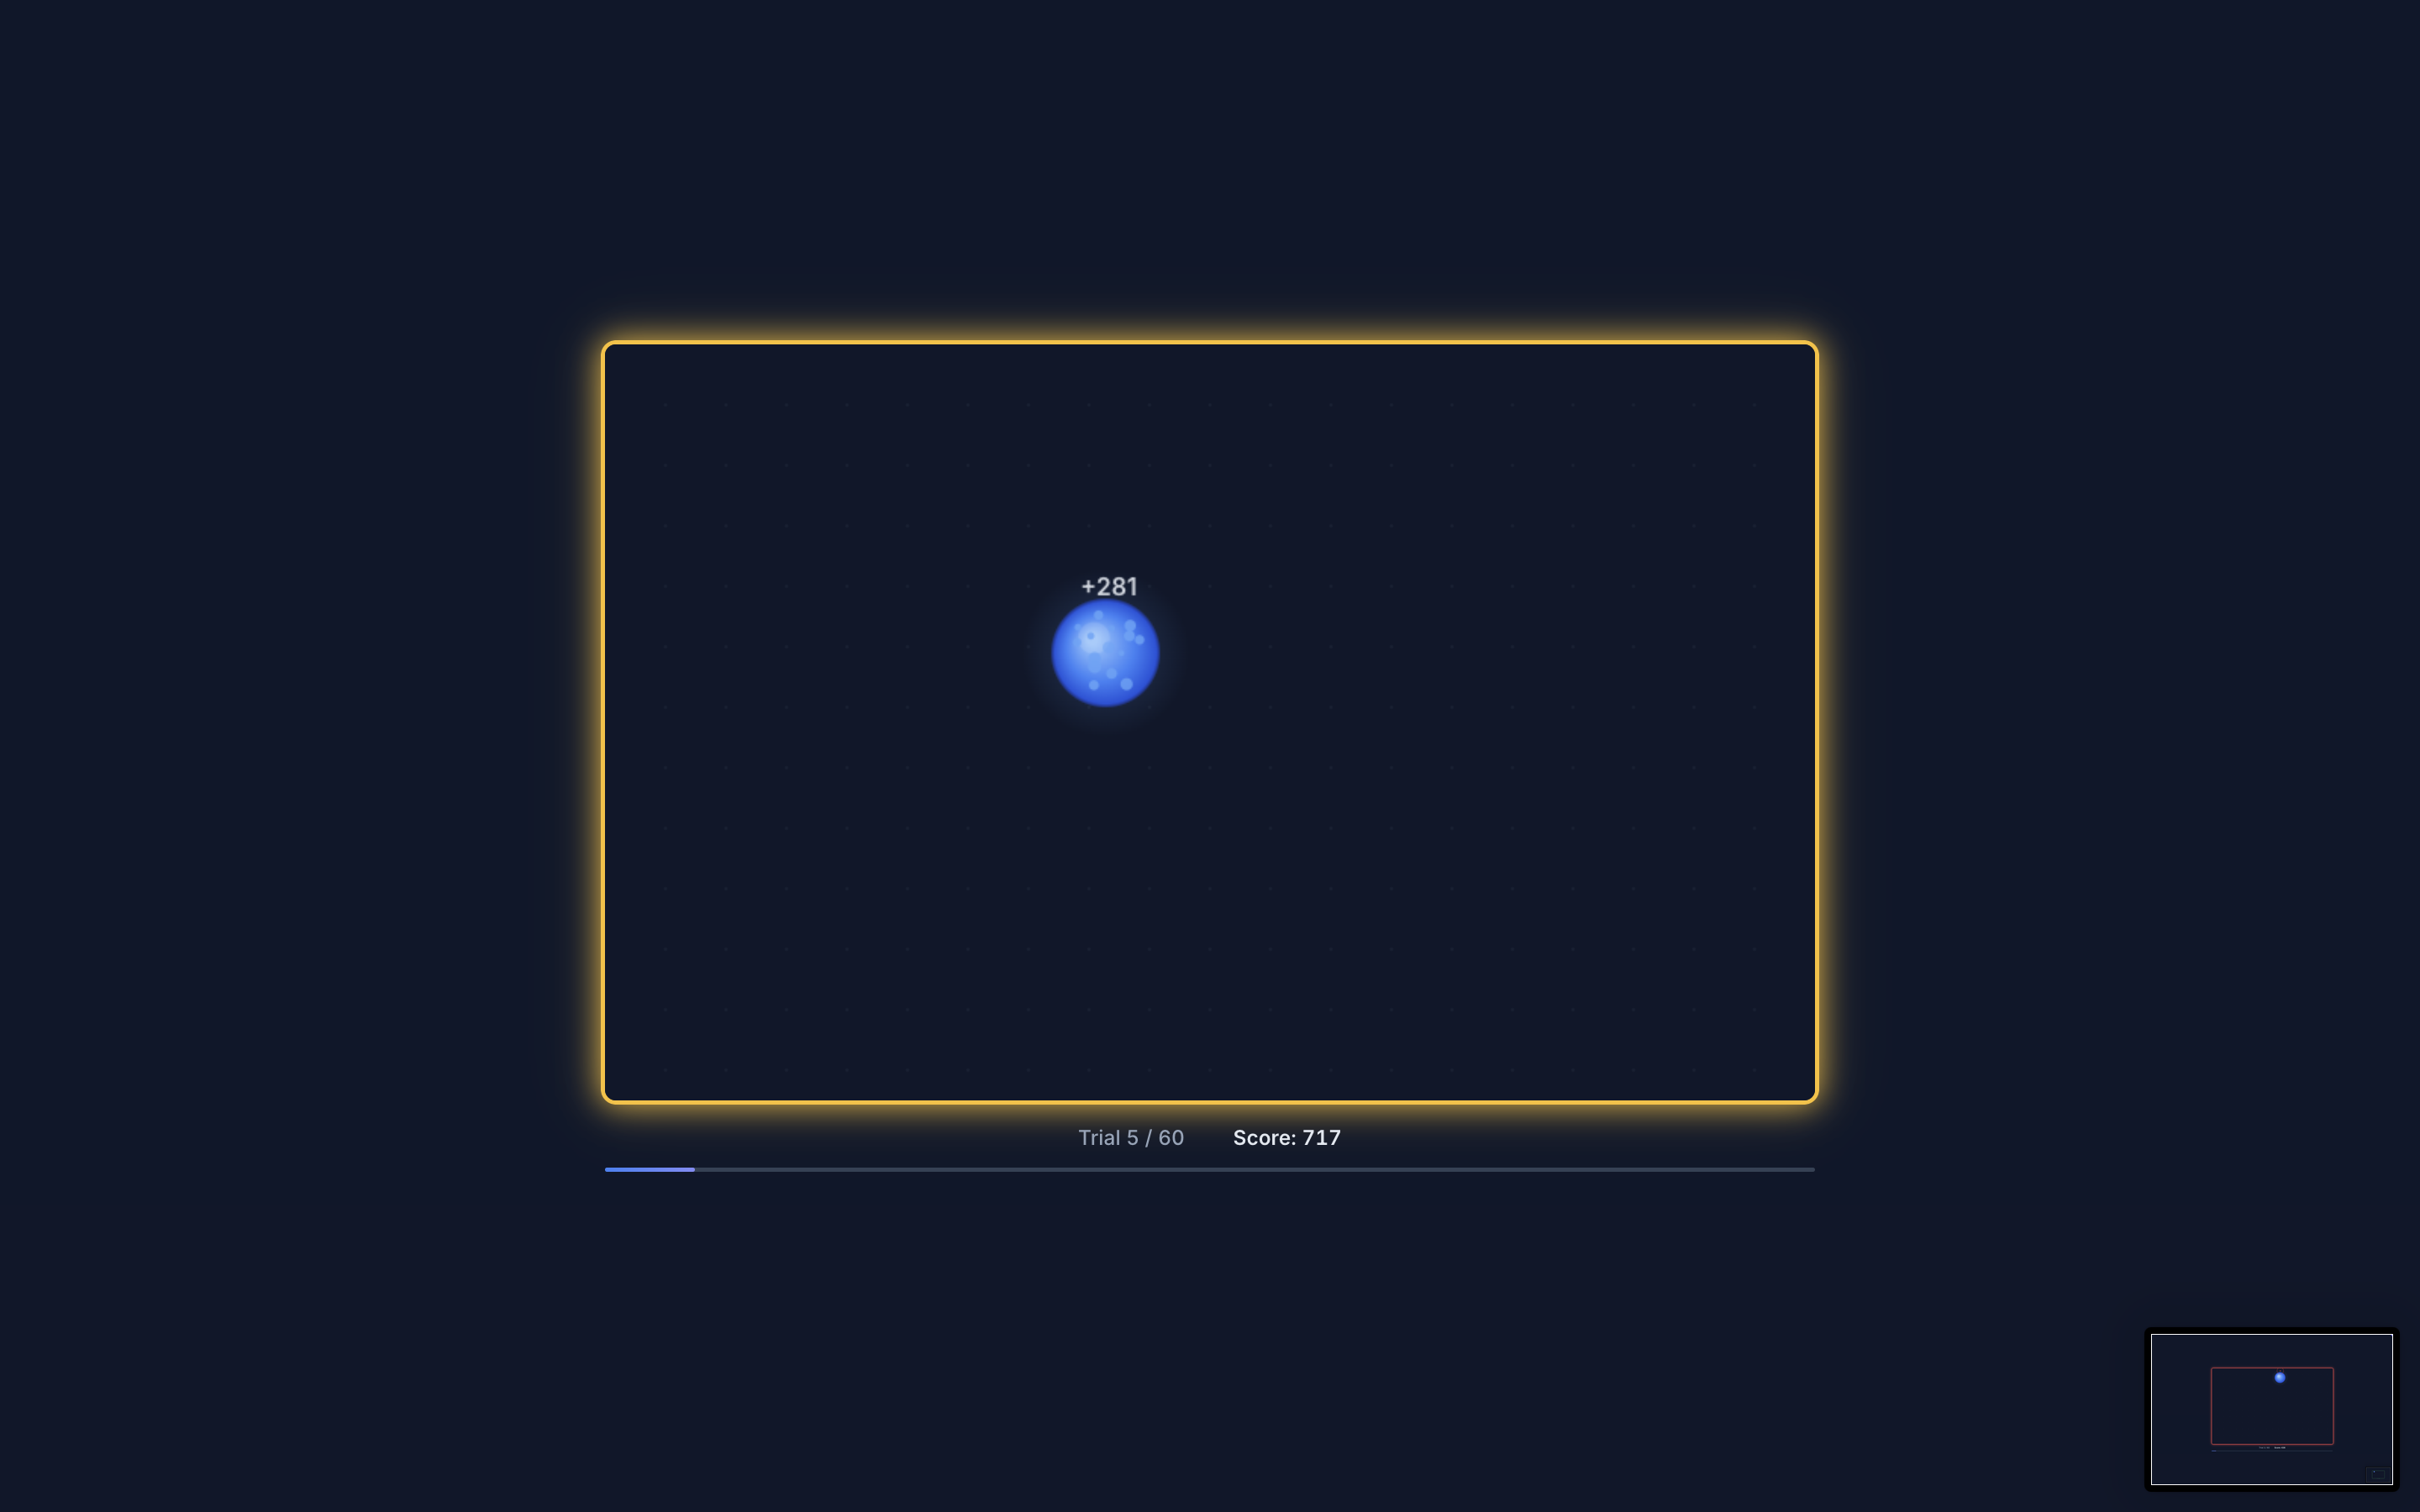
\includegraphics[width=\textwidth]{hit_gold_feedback_visual.png}
  \caption{Gold (fast)}
\end{subfigure}
\hfill
\begin{subfigure}[t]{0.30\textwidth}
  \centering
  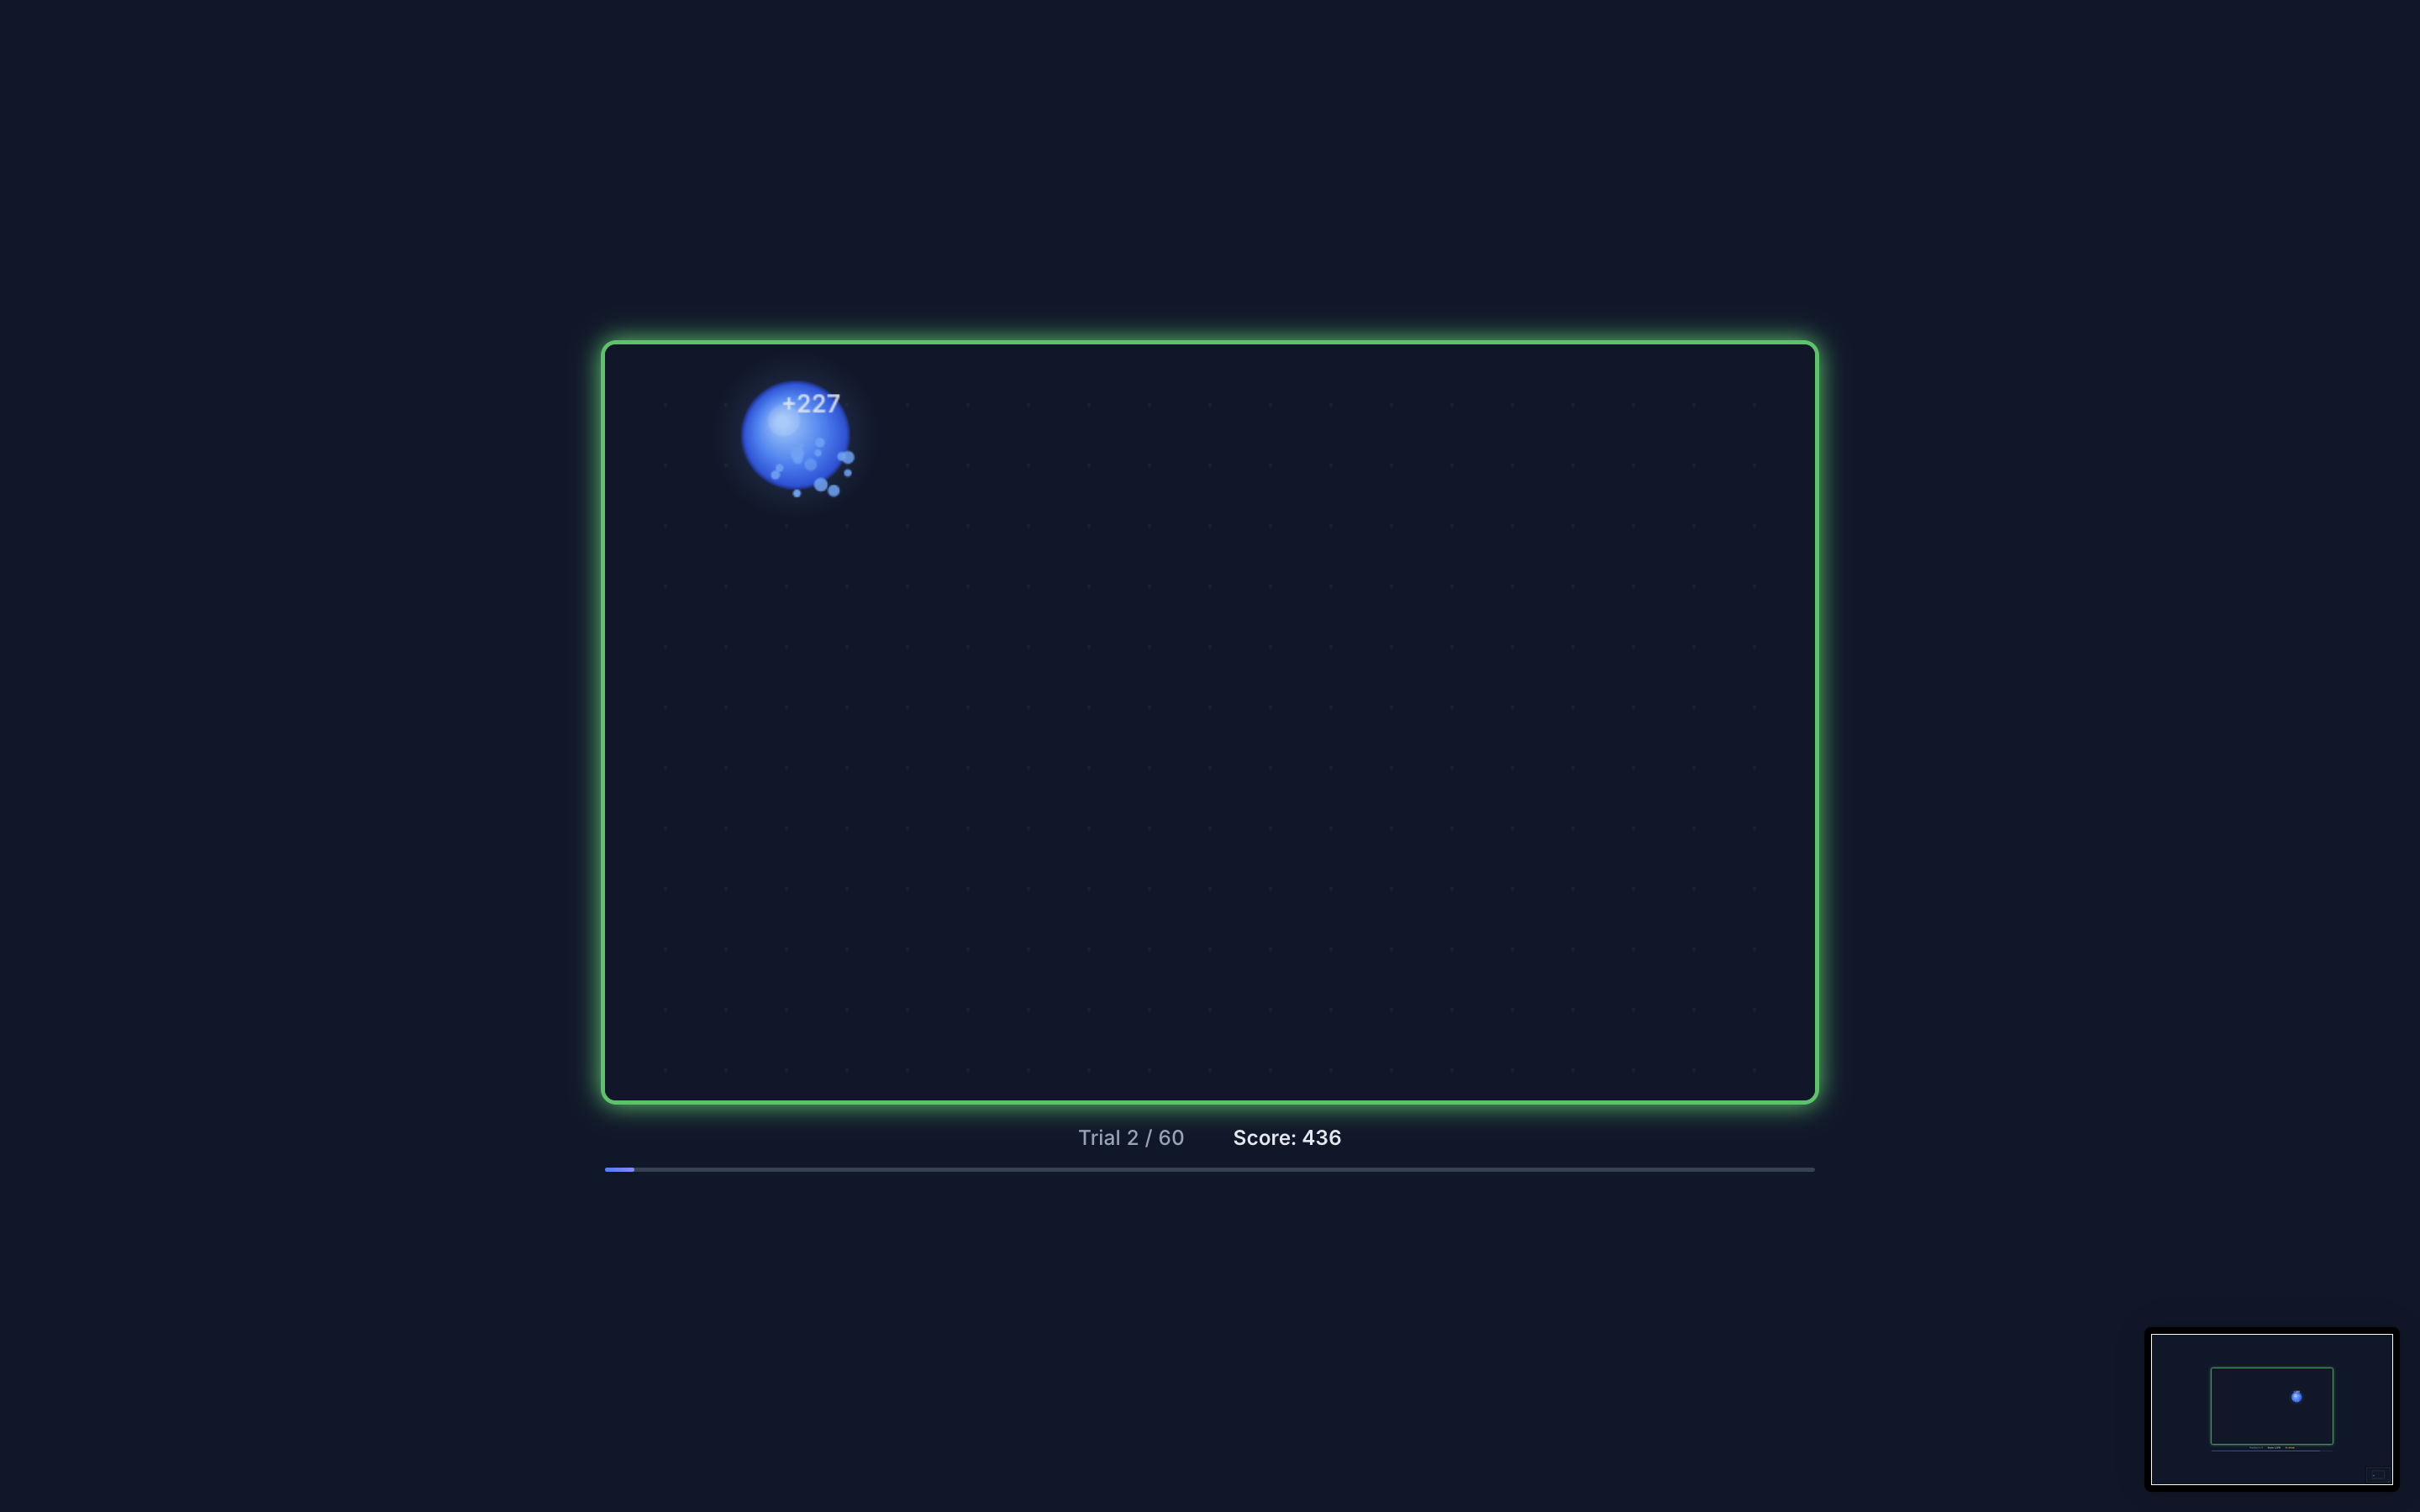
\includegraphics[width=\textwidth]{green_feedback_visual.png}
  \caption{Green (slow)}
\end{subfigure}
\hfill
\begin{subfigure}[t]{0.30\textwidth}
  \centering
  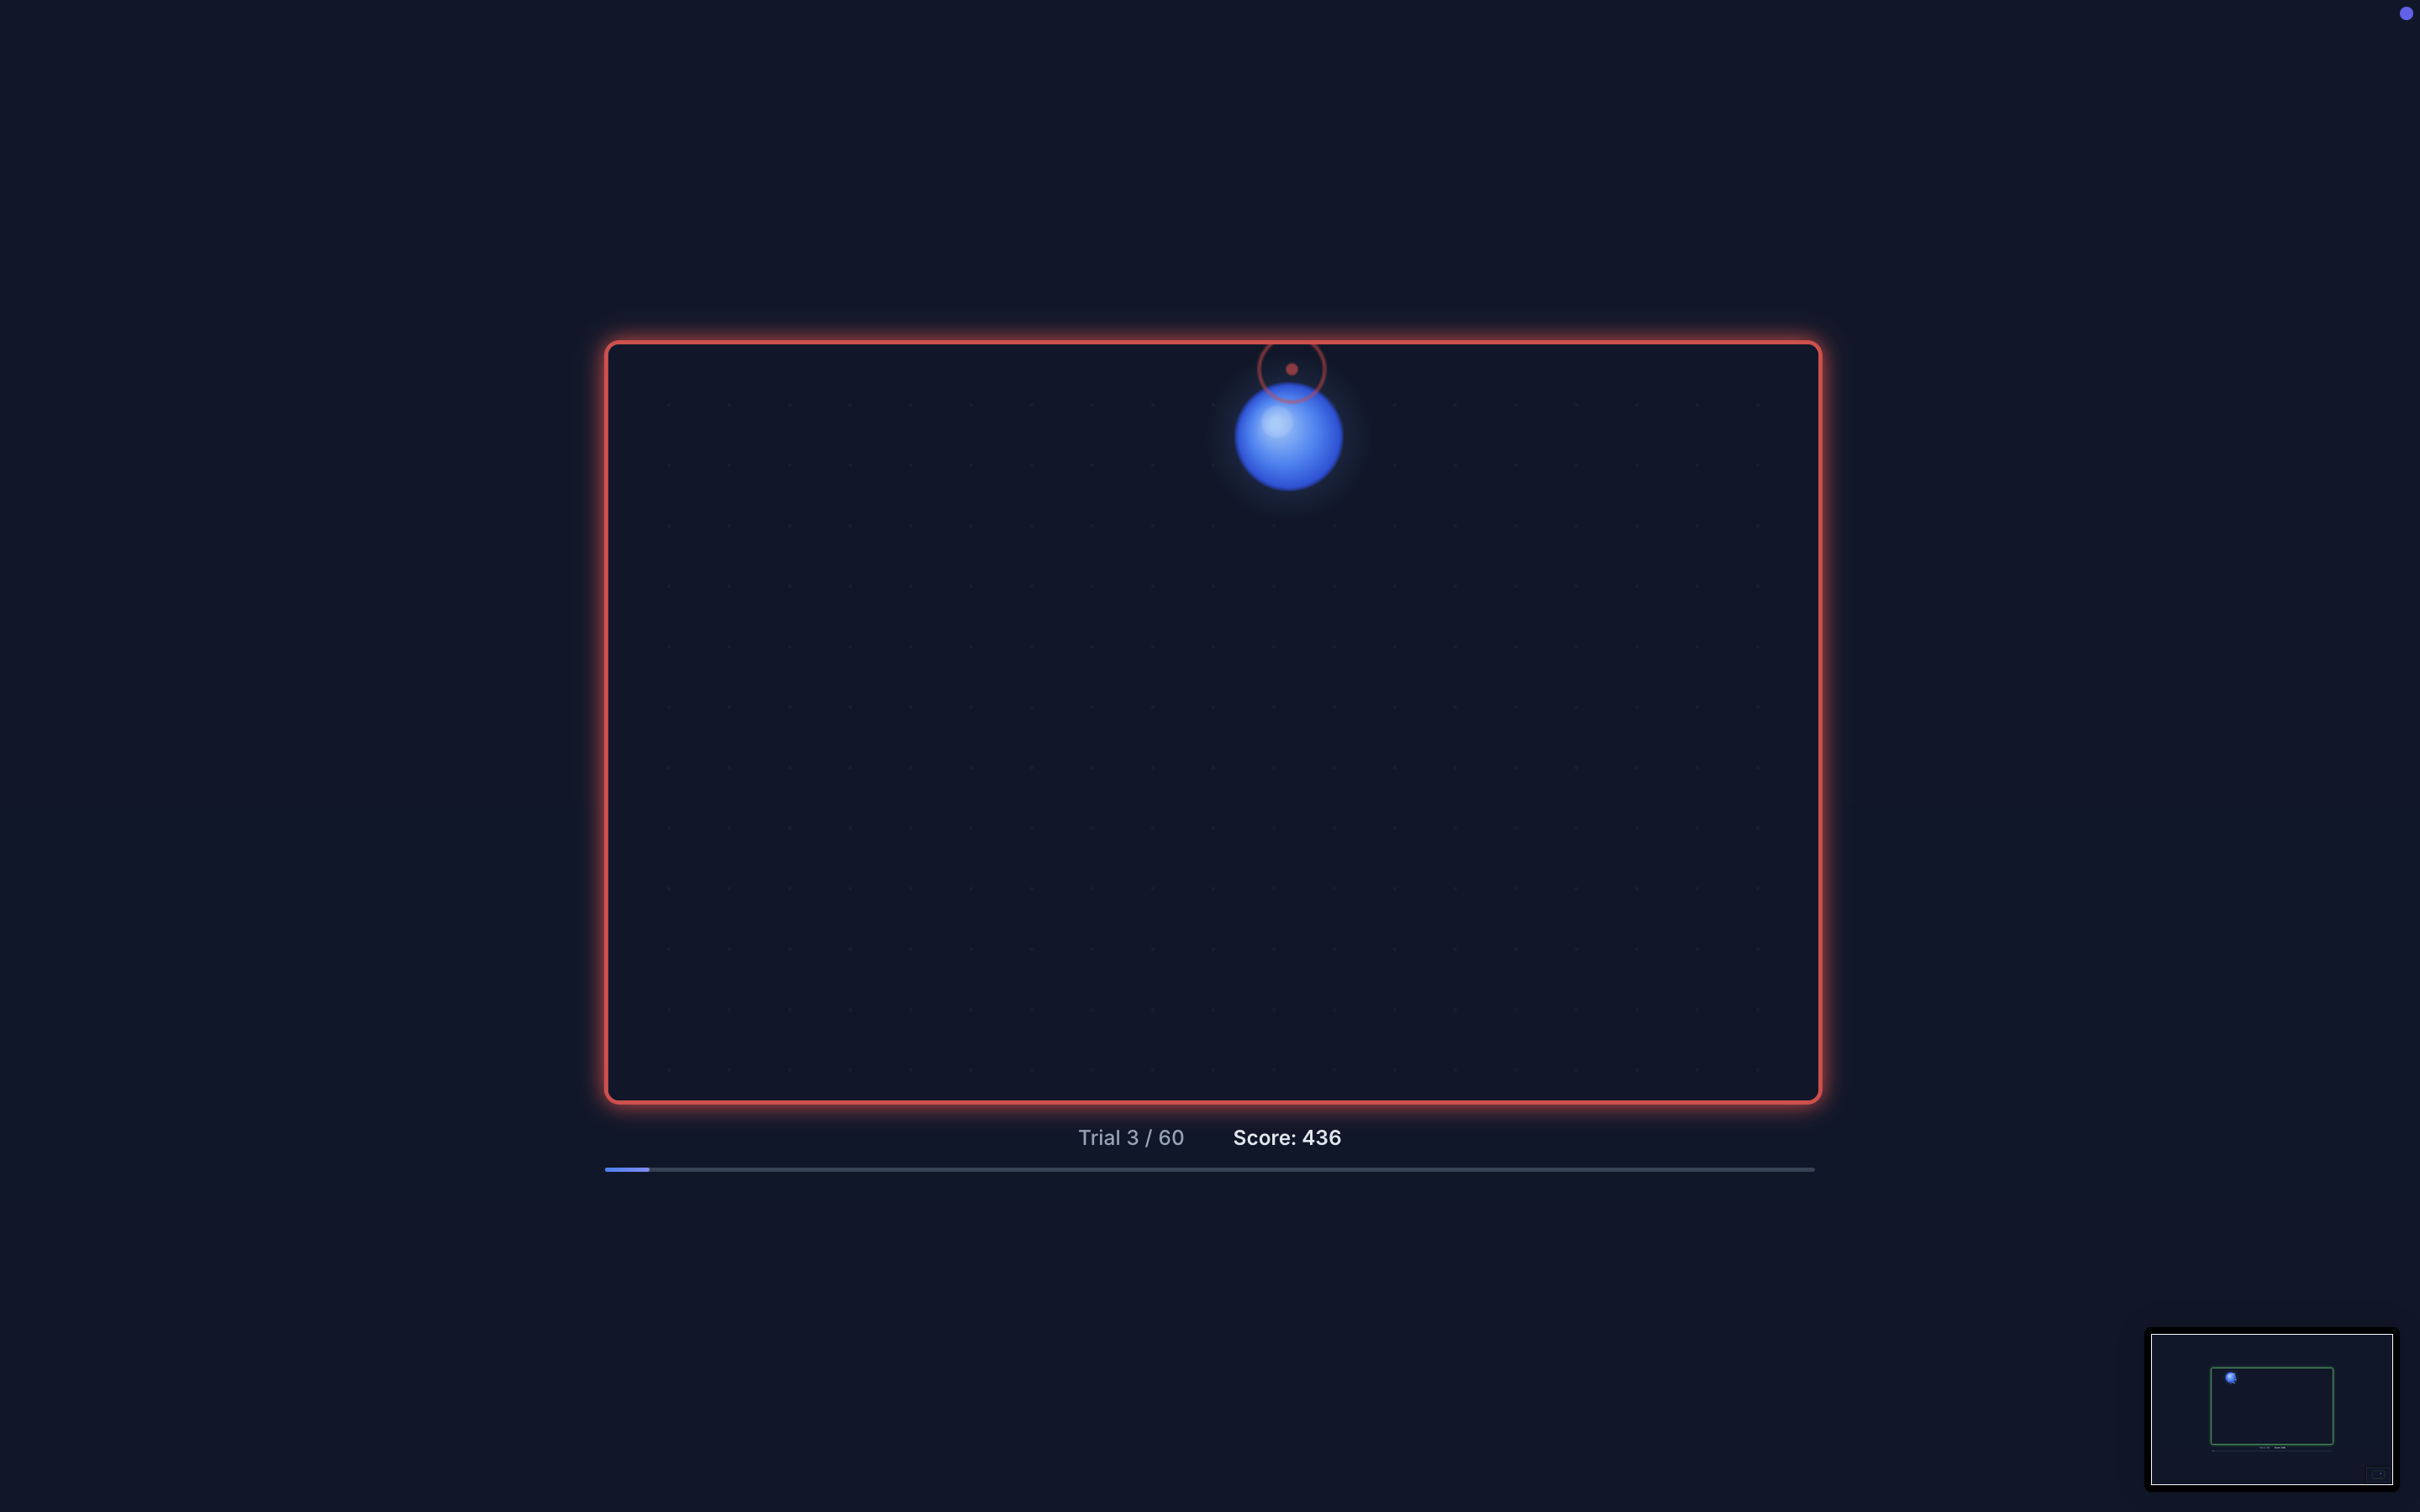
\includegraphics[width=\textwidth]{miss_feedback_visual.png}
  \caption{Red + shake (miss)}
\end{subfigure}
\caption{Visual feedback states. The gold vs.\ green distinction created a speed incentive.}
\label{fig:feedback_states}
\end{figure}

\subsection{Independent Variable}

Feedback type was within-subject with two levels:

\textbf{Visual.} Border glow; gold ($<$600\,ms), green ($\geq$600\,ms), or red + shake (miss). 150\,ms duration.

\textbf{Auditory.} Pure tones; 880\,Hz (fast hit), 440\,Hz (slow hit), 180\,Hz (miss). 200\,ms duration.

Both conditions conveyed identical three-level information. The on-screen HUD (trial counter, score, streak) was identical in both conditions. This addresses the proposal feedback, which noted an information asymmetry in the original design.

\subsection{Dependent Variables}

\textbf{DV\textsubscript{1}: Reaction time} (ms), target onset to click.

\textbf{DV\textsubscript{2}: Radial error} (px), Euclidean distance from click to target center. Hit = error $\leq$ 35\,px.

\subsection{Procedure}

\vspace{4pt}
\noindent
\fbox{\parbox{0.95\textwidth}{\small
Consent $\;\to\;$ Instructions $\;\to\;$ 5 practice trials $\;\to\;$ \textbf{Block 1} (30 or 60 trials) $\;\to\;$ Break $\;\to\;$ \textbf{Block 2} $\;\to\;$ End screen
}}
\vspace{4pt}

Condition order was randomized per participant. Target positions were randomized. A gamification system (scoring, particle effects, and a leaderboard) was used to boost engagement and recruitment.

\subsection{Potential Biases}

Convenience sampling limits generalizability. Device variability was controlled as a covariate in the H\textsubscript{3} regression. Audio environment was uncontrolled. Four participants completed the experiment twice; each attempt was treated as a separate observation.


% ═══ 4. ANALYSIS ══════════════════════════════════════════════
\section{Analysis}

\subsection{Data Cleaning}

Only participants who completed the full 60-trial protocol were included ($N = 41$ of 72 total). Trials with RT $< 150$\,ms or $> 8{,}000$\,ms were excluded. The remaining 4{,}919 trials were aggregated to per-participant means for each condition, yielding 41 paired observations.

\subsection{Assumption Checks}

Normality of within-subject differences was assessed with the Shapiro--Wilk test (Week 10: goodness of fit). RT differences were normal ($W = 0.980$, $p = .304$), so a paired $t$-test was appropriate for H\textsubscript{1}. Error differences were non-normal ($W = 0.420$, $p < .001$) due to heavy tails, so a Wilcoxon signed-rank test was used for H\textsubscript{2}. QQ plots are in Appendix~A.

\subsection{Hypothesis Tests}

\textbf{H\textsubscript{1} (Speed).} Our original prediction, based on MRT, was that auditory feedback would be faster. The data showed the opposite. We used a \emph{two-tailed} paired $t$-test (hypothesis testing, confidence intervals) because our directional prediction was reversed:
\vspace{-4pt}
\begin{align*}
  H_0 &: \mu_{\text{vis}} = \mu_{\text{aud}} &\quad H_1 &: \mu_{\text{vis}} \neq \mu_{\text{aud}}
\end{align*}

\textbf{H\textsubscript{2} (Accuracy).} One-tailed Wilcoxon signed-rank test (nonparametric alternative, normality violated):
\vspace{-4pt}
\begin{align*}
  H_0 &: \text{median}(d_{\text{error}}) \leq 0 &\quad H_1 &: \text{median}(d_{\text{error}}) > 0
\end{align*}
where $d = \bar{e}_{\text{vis}} - \bar{e}_{\text{aud}}$ per participant.

\textbf{H\textsubscript{3} (SAT structure).} Multiple linear regression with interaction (Week 12--13):
\[
  \text{error} = \beta_0 + \beta_1 \!\cdot\! \text{RT} + \beta_2 \!\cdot\! \text{condition} + \beta_3 \!\cdot\! (\text{RT} \times \text{condition}) + \varepsilon
\]
A significant $\beta_3$ indicates different SAT slopes. Supplemented with Pearson correlations (Week 2--3) and simple linear regression per condition (Week 11).

All tests used $\alpha = 0.05$, setting the Type~I error rate (false positive) at 5\%. Cohen's $d$ is reported for paired comparisons. The shift from 30 to 60 trials was motivated by reducing Type~II error (false negative): the 30-trial cohort lacked sufficient power to detect the small within-subject effects (see Appendix~\ref{app:30v60}).


% ═══ 5. RESULTS ═══════════════════════════════════════════════
\section{Results}

\subsection{Descriptive Statistics}

Table~\ref{tab:dvs} summarizes the two dependent variables. Visual feedback was associated with significantly faster responses ($-18.5$\,ms, $p = .047$) and significantly greater error ($+1.0$\,px, $p = .026$), consistent with a speed-accuracy tradeoff.

\begin{table}[H]
\centering
\caption{Performance by feedback condition ($N = 41$, 60-trial participants only). Per-participant means $\pm$ SD.}
\label{tab:dvs}
\small
\begin{tabular}{lcccccc}
\toprule
& \multicolumn{2}{c}{\textbf{Visual}} & \multicolumn{2}{c}{\textbf{Auditory}} & \textbf{Diff} & \textbf{$p$} \\
\cmidrule(lr){2-3} \cmidrule(lr){4-5}
& $M$ & $SD$ & $M$ & $SD$ & & \\
\midrule
RT (ms) & 675 & 135 & 693 & 142 & $-18.5$ & .047 \\
Error (px) & 13.9 & 5.6 & 12.9 & 4.5 & $+1.0$ & .026 \\
Hit Rate (\%) & 96.0 & 5.7 & 97.0 & 4.3 & $-1.0$ & \\
RT $\sigma$ (ms) & 134.9 & & 142.4 & & $-7.5$ & \\
\bottomrule
\end{tabular}
\end{table}

\subsection{Reaction Time}

\begin{figure}[H]
\centering
\begin{subfigure}[t]{0.48\textwidth}
  \centering
  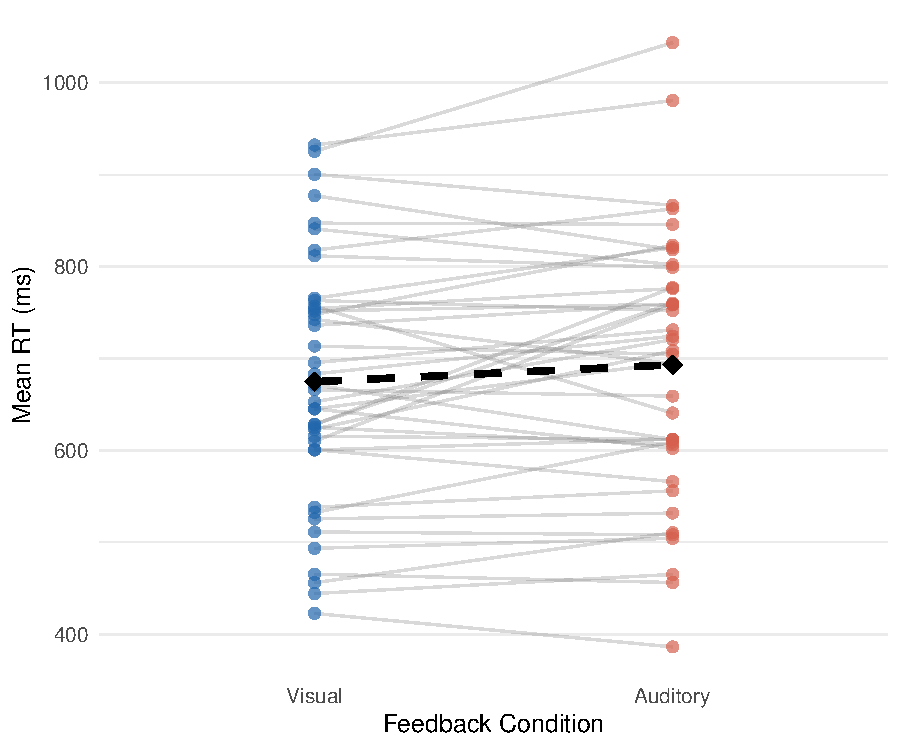
\includegraphics[width=\textwidth]{rt_spaghetti.pdf}
  \caption{Paired RT. Grey lines = individuals. Diamond = grand mean.}
  \label{fig:spaghetti}
\end{subfigure}
\hfill
\begin{subfigure}[t]{0.48\textwidth}
  \centering
  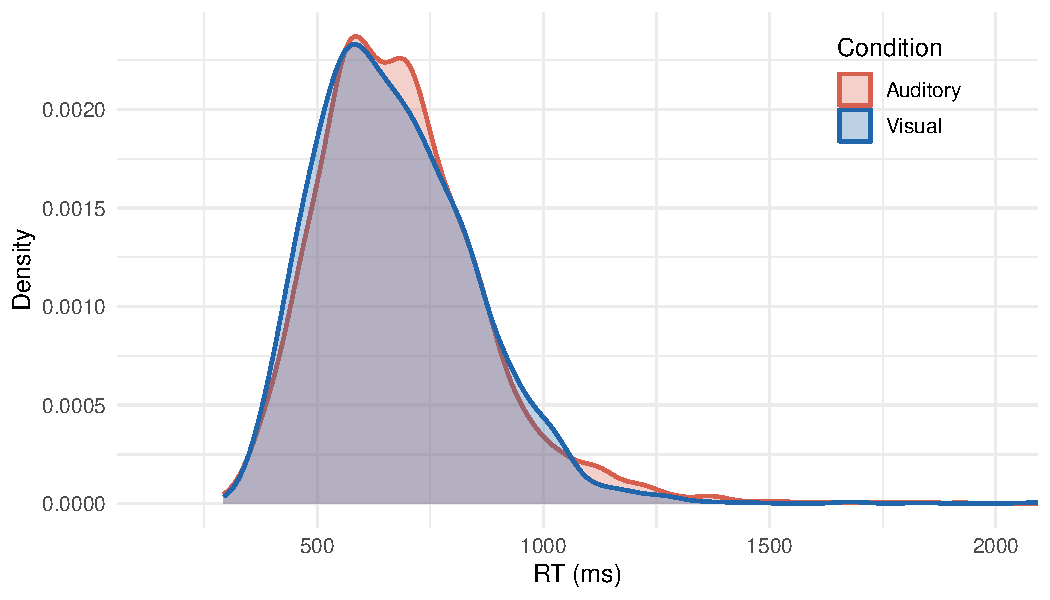
\includegraphics[width=\textwidth]{rt_density.pdf}
  \caption{RT distributions. Visual is tighter, peaking near the 600\,ms gold threshold.}
  \label{fig:density}
\end{subfigure}
\caption{Reaction time by condition. Individual variation is large ($SD = 56.5$\,ms for paired differences), which is why H\textsubscript{1} did not reach significance despite a 9.7\,ms mean difference.}
\end{figure}

\textbf{H\textsubscript{1} result.} Paired $t$-test: $t(40) = -2.05$, $p = .047$, 95\% CI $[-36.7,\ -0.2]$\,ms, $d = -0.32$. We reject $H_0$: visual feedback produced significantly faster responses.

\subsection{Radial Error}

\textbf{H\textsubscript{2} result.} Wilcoxon signed-rank: $V = 580$, $p = .026$ (one-tailed), $d = 0.27$. Significant: visual feedback produced greater radial error, consistent with a speed-accuracy tradeoff.

\subsection{Speed--Accuracy Tradeoff Structure}

The linear correlations between RT and error are weak ($r_{\text{vis}} = -.193$, $r_{\text{aud}} = -.154$). Rather than a clean linear tradeoff, the data shows a Pareto-like boundary pattern (Figure~\ref{fig:sat_density}): trials cluster in the fast-and-accurate region, with outliers spreading along either the high-error or high-RT axis, but almost no trials are both slow \emph{and} inaccurate. This suggests a performance frontier rather than a simple linear SAT.

\begin{figure}[H]
\centering
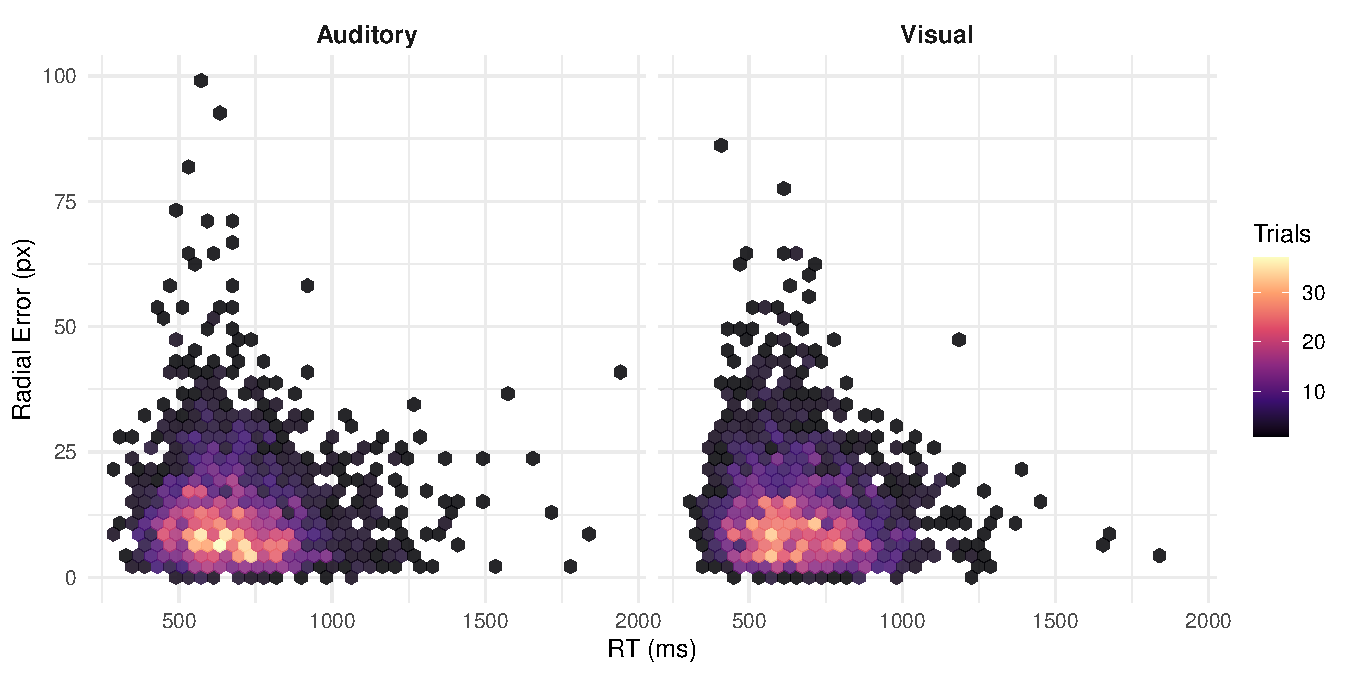
\includegraphics[width=0.9\textwidth]{sat_density.pdf}
\caption{2D density of RT vs.\ error by condition. Trials cluster in the low-RT, low-error region. The near-empty upper-right quadrant (slow and inaccurate) reveals a Pareto-like performance boundary.}
\label{fig:sat_density}
\end{figure}

\textbf{H\textsubscript{3} result.} With device type included as a covariate, the multiple regression interaction was highly significant: $\beta_3 = -0.0106$, $t(4913) = -5.49$, $p < .001$. The visual slope ($b = -0.009$) was steeper than auditory ($b = -0.001$, $R^2 = .001$), confirming that visual feedback amplifies the linear component of the speed-accuracy relationship. The model $R^2 = .032$ is modest, consistent with the Pareto-like boundary pattern dominating the data rather than a clean linear trend.

\textbf{Individual-level cross-condition SAT.} Beyond the population-level tests, the SAT can also be examined at the individual level. Figure~\ref{fig:ind_sat} plots each participant's RT change (visual minus auditory) against their error change. The correlation is $r = -0.193$ ($p = .104$, 95\% CI $[-0.41,\ 0.04]$): participants who became faster under visual tended to become slightly less accurate. Though not significant at $\alpha = 0.05$, the direction is consistent with a speed-accuracy tradeoff operating \emph{across conditions within individuals}, even when the population averages wash it out.

The scatter also shows a boundary pattern consistent with the trial-level data: participants cluster in the fast-and-accurate or slow-and-precise quadrants, with few in the slow-and-inaccurate quadrant. This reciprocal-like shape suggests a performance ceiling where both speed and accuracy cannot degrade simultaneously.

\begin{figure}[H]
\centering
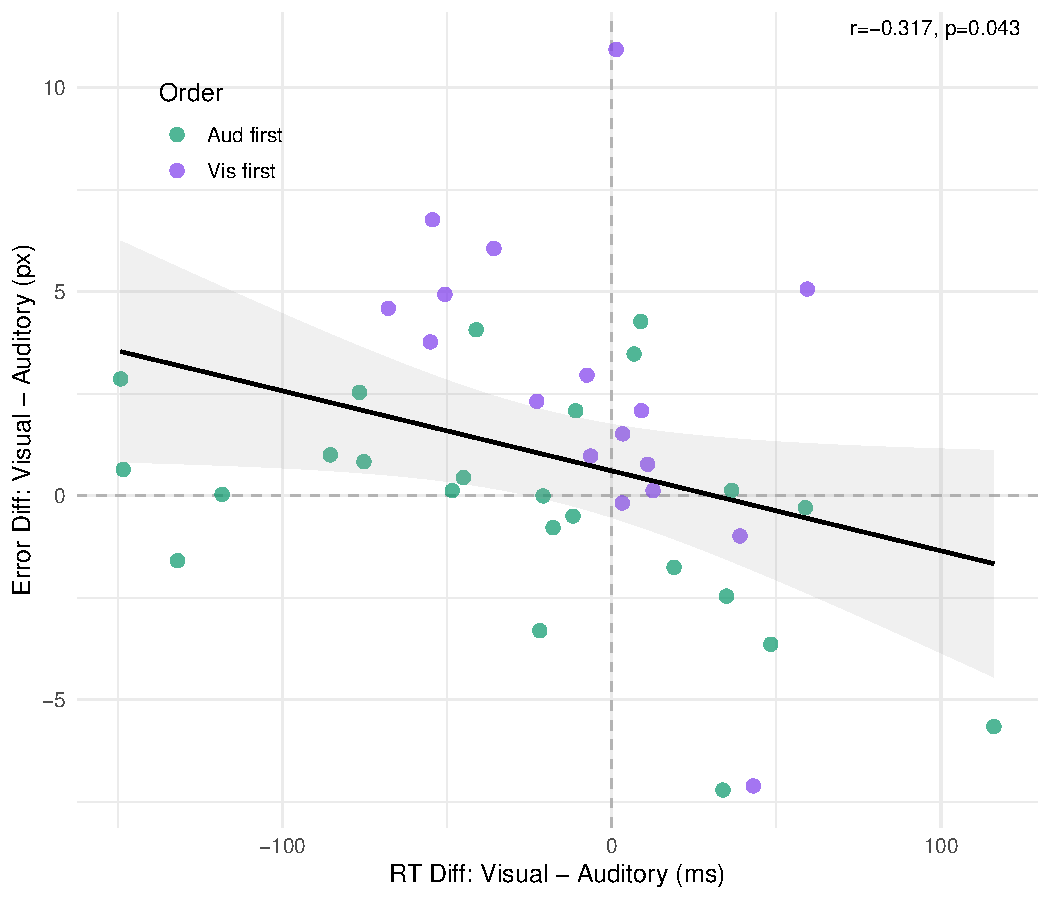
\includegraphics[width=0.65\textwidth]{individual_sat.pdf}
\caption{Individual-level SAT across conditions. Each point = one participant. Participants below the diagonal (lower-left) sped up under visual but paid an accuracy cost. $r = -0.193$, $p = .104$.}
\label{fig:ind_sat}
\end{figure}

\subsection{Covariates}

\begin{table}[H]
\centering
\caption{Performance by input device and gaming frequency.}
\label{tab:covariates}
\begin{tabular}{lcccc}
\toprule
& $N$ & Mean RT (ms) & Mean Error (px) & Hit Rate (\%) \\
\midrule
\multicolumn{5}{l}{\textit{Input Device}} \\
\quad Mouse & 18 & 588 & 12.2 & 96.9 \\
\quad Trackpad & 16 & 792 & 14.8 & 95.8 \\
\quad Other & 7 & 681 & 13.1 & 97.0 \\[4pt]
\multicolumn{5}{l}{\textit{Gaming Frequency}} \\
\quad Daily & 9 & 598 & 10.8 & 99.4 \\
\quad Weekly & 10 & 680 & 14.0 & 95.7 \\
\quad Never & 9 & 695 & 13.5 & 97.0 \\
\quad Rarely & 13 & 739 & 14.7 & 94.9 \\
\bottomrule
\end{tabular}
\end{table}

Mouse users were 204\,ms faster than trackpad users (588 vs.\ 792\,ms) but had similar hit rates, a device-level SAT. Device type was included as a covariate in the H\textsubscript{3} regression to control for this. Daily gamers were the fastest (598\,ms) \emph{and} most accurate (99.4\%), while rare gamers were slowest (739\,ms) and least accurate (94.9\%). Trackpad users showed a stronger visual feedback effect ($d = -0.34$, $p = .065$) than mouse users ($d = -0.08$, $p = .70$), suggesting the modality effect is larger when the task is harder.

\subsection{Tilt Effect (Error Cascading)}

When a participant missed, the probability of missing the \emph{next} trial was 15.0\% (25/167), compared to just 3.0\% (139/4{,}670) after a hit. That is a \textbf{5$\times$ increase}, $\chi^2(1) = 67.2$, $p < .001$. Errors cascade: a single miss temporarily disrupts focus or motor calibration, triggering further misses. This ``tilt'' effect (borrowing the poker term for emotion-driven errors) operated in both conditions and is visualized in Table~\ref{tab:tilt}.

\begin{table}[H]
\centering
\caption{Tilt effect: probability of miss conditional on previous trial outcome.}
\label{tab:tilt}
\begin{tabular}{lcc}
\toprule
& \textbf{Next = Hit} & \textbf{Next = Miss} \\
\midrule
Previous = Hit & 4{,}531 (97.0\%) & 139 (3.0\%) \\
Previous = Miss & 142 (85.0\%) & 25 (15.0\%) \\
\bottomrule
\end{tabular}
\end{table}

\subsection{Spatial Click Patterns}

On misses ($n = 171$), there was a systematic spatial bias: participants clicked an average of 5.4\,px below and 1.3\,px to the right of the target, likely reflecting cursor hotspot position or hand biomechanics.

Edge targets (distance from canvas center $\geq 150$\,px) were harder: mean RT of 727\,ms vs.\ 666\,ms for center targets ($p < .001$), with a slightly lower hit rate (94.9\% vs.\ 95.8\%). This confirms a Fitts' Law-like effect. The full click scatter is in Appendix~B (Figure~B.1).

\subsection{Additional Controls}

Condition order was randomized per participant. Counterbalancing was effective: no significant difference in overall RT between Visual-first and Auditory-first groups, $t = 0.40$, $p = .690$. Visual participants slowed down 65.5\,ms after a miss vs.\ only 17.4\,ms for auditory, suggesting visual feedback makes failure more salient (Figure~\ref{fig:postmiss} in Appendix).


% ═══ 6. CONCLUSION ════════════════════════════════════════════
\section{Conclusion}

All three hypotheses were supported in the 60-trial cohort. Visual feedback produced significantly faster responses (H\textsubscript{1}: $p = .047$, $d = -0.32$), significantly greater radial error (H\textsubscript{2}: $p = .026$, $d = 0.27$), and a significantly steeper SAT slope (H\textsubscript{3}: $p < .001$). Notably, when the analysis included the 30-trial participants ($N = 72$), none of these effects reached significance (H\textsubscript{1}: $p = .151$; H\textsubscript{2}: $p = .184$; H\textsubscript{3}: $p = .023$), demonstrating the importance of sufficient trial counts for detecting within-subject effects. This motivated our shift from 30 to 60 trials per block during the experiment design.

The MRT prediction, that auditory feedback should reduce interference, was not supported. Instead, the visual condition's gold/green glow created a speed incentive: participants could \emph{see} whether they were ``fast'' and were visibly frustrated at getting green instead of gold. This speed-chasing was absent in the auditory condition. MRT's interference framework is incomplete: modality affects not only attentional load but also \emph{motivation}.

The tilt effect ($\chi^2 = 67.2$, $p < .001$) demonstrates that trial independence cannot be assumed in sequential motor tasks: a single miss increases the next-trial miss probability by 5$\times$.

\textbf{Practical implications.} Visual feedback may inadvertently create speed pressure in safety-critical interfaces; auditory feedback may better preserve accuracy.

\textbf{Limitations.} Effect sizes were small to medium ($d = 0.27$--$0.32$). Accuracy was near ceiling ($\sim$96\%), limiting the range of detectable error differences. The linear SAT model explains only 3.2\% of variance; the Pareto-like boundary pattern suggests a constraint envelope rather than a linear function. Device variability was controlled as a covariate in the regression but still introduced noise in the paired tests. Convenience sampling (all 18--24 university students) limits generalizability. The visual border glow is inherently more salient than a tone; our results speak to feedback ``as deployed'' rather than pure modality.

\textbf{Lessons learned.} Counterbalancing confirmed no order effect ($p = .960$). Gamification boosted engagement without biasing within-subject comparisons. The gold/green speed indicator, intended as neutral feedback, became a performance incentive, which is itself evidence that visual feedback drives speed-chasing behavior. Future work should manipulate feedback salience independently of modality to disentangle interference and motivational effects.


% ═══ REFERENCES ════════════════════════════════════════════════
\section*{References}
{\small
\begin{enumerate}[label={[\arabic*]},leftmargin=1.5em,itemsep=2pt]
  \item C.\,D.\ Wickens, ``Multiple resources and performance prediction,'' \emph{Theor.\ Issues Ergon.\ Sci.}, 3(2), 159--177, 2002.
  \item C.\,D.\ Wickens et al., \emph{Engineering Psychology and Human Performance}, 4th ed., Routledge, 2015.
  \item J.\ Sweller, ``Cognitive load during problem solving,'' \emph{Cognitive Science}, 12(2), 257--285, 1988.
  \item P.\,M.\ Fitts, ``Information capacity of the human motor system,'' \emph{J.\ Exp.\ Psychol.}, 47(6), 381--391, 1954.
  \item I.\,S.\ MacKenzie, ``Fitts' law as a research and design tool in HCI,'' \emph{Hum.-Comput.\ Interact.}, 7(1), 91--139, 1992.
  \item R.\,P.\ Heitz, ``The speed-accuracy tradeoff: history, physiology, methodology, and behavior,'' \emph{Front.\ Neurosci.}, 8, 150, 2014.
  \item M.\ Akamatsu et al., ``Tactile, auditory, and visual feedback in a pointing task,'' \emph{Ergonomics}, 38(4), 816--827, 1995.
  \item R.\ Sigrist et al., ``Augmented visual, auditory, haptic, and multimodal feedback in motor learning,'' \emph{Psychon.\ Bull.\ Rev.}, 20(1), 21--53, 2013.
\end{enumerate}
}


% ═══ APPENDICES ════════════════════════════════════════════════
\newpage
\appendix

\section{Assumption Checks}

\begin{itemize}
  \item RT differences: $W = 0.980$, $p = .304$ : normal. Paired $t$-test appropriate.
  \item Error differences: $W = 0.420$, $p < .001$ : non-normal. Wilcoxon used.
\end{itemize}

\begin{figure}[H]
\centering
\begin{subfigure}[t]{0.48\textwidth}
  \centering
  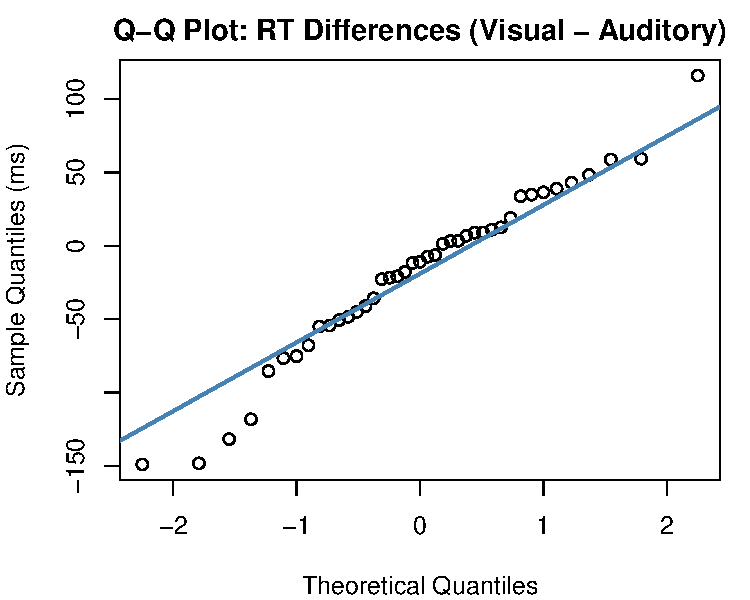
\includegraphics[width=\textwidth]{qq_rt.pdf}
  \caption{RT differences:approximately normal.}
\end{subfigure}
\hfill
\begin{subfigure}[t]{0.48\textwidth}
  \centering
  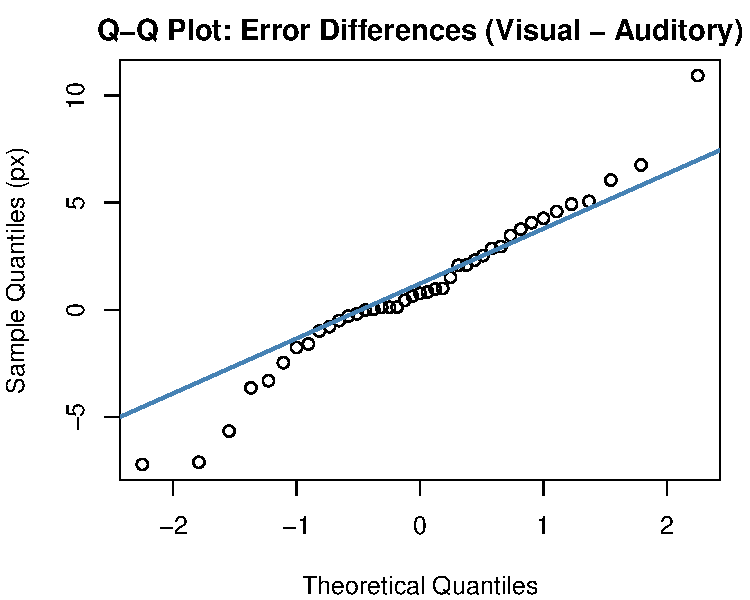
\includegraphics[width=\textwidth]{qq_error.pdf}
  \caption{Error differences:heavy tails, non-normal.}
\end{subfigure}
\caption{QQ plots for within-subject differences (visual $-$ auditory).}
\end{figure}

\begin{figure}[H]
\centering
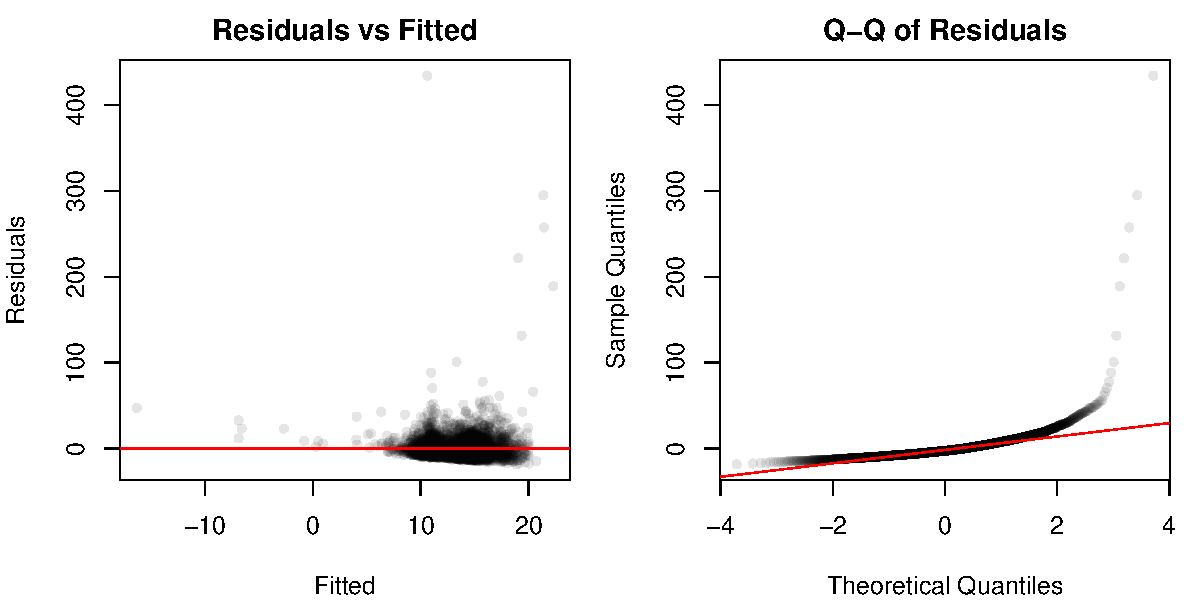
\includegraphics[width=0.85\textwidth]{residuals.pdf}
\caption{Residual diagnostics for the SAT interaction model. Funnel pattern expected with bounded error; heavy right tail from large misses.}
\end{figure}


\section{Additional Figures}

\begin{figure}[H]
\centering
\begin{subfigure}[t]{0.48\textwidth}
  \centering
  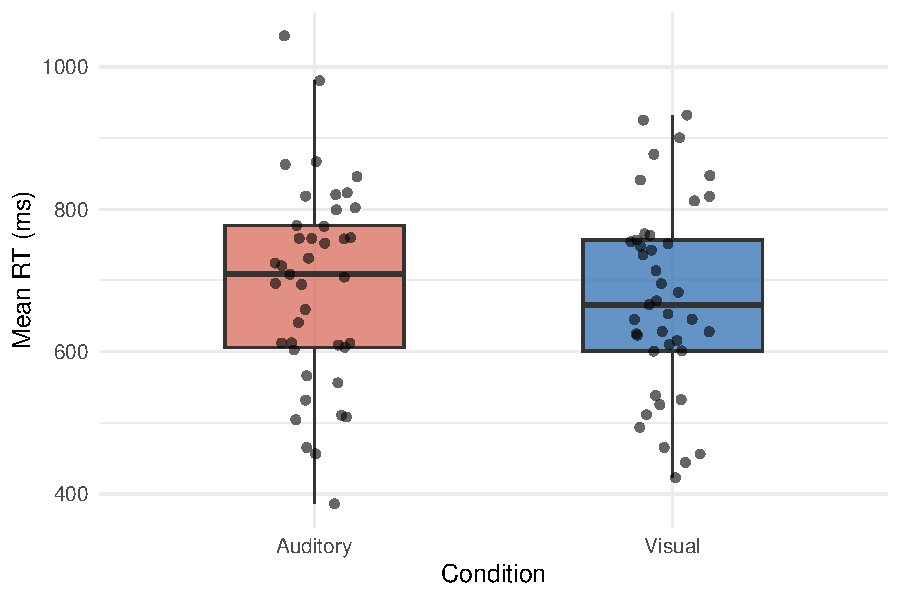
\includegraphics[width=\textwidth]{rt_boxplot.pdf}
  \caption{RT by condition with individual points.}
\end{subfigure}
\hfill
\begin{subfigure}[t]{0.48\textwidth}
  \centering
  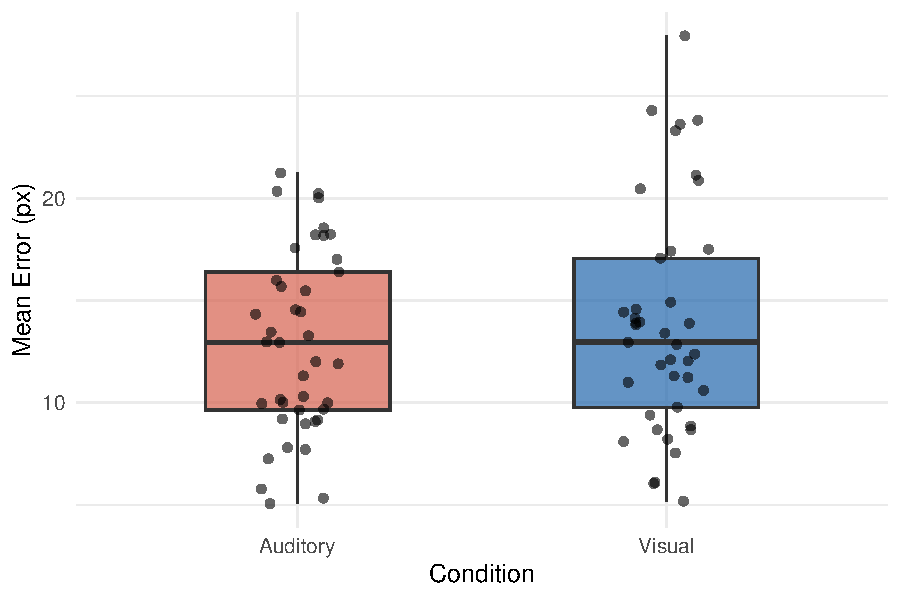
\includegraphics[width=\textwidth]{error_boxplot.pdf}
  \caption{Radial error by condition.}
\end{subfigure}
\caption{Boxplots of per-participant means by feedback condition.}
\end{figure}

\begin{figure}[H]
\centering
\begin{subfigure}[t]{0.48\textwidth}
  \centering
  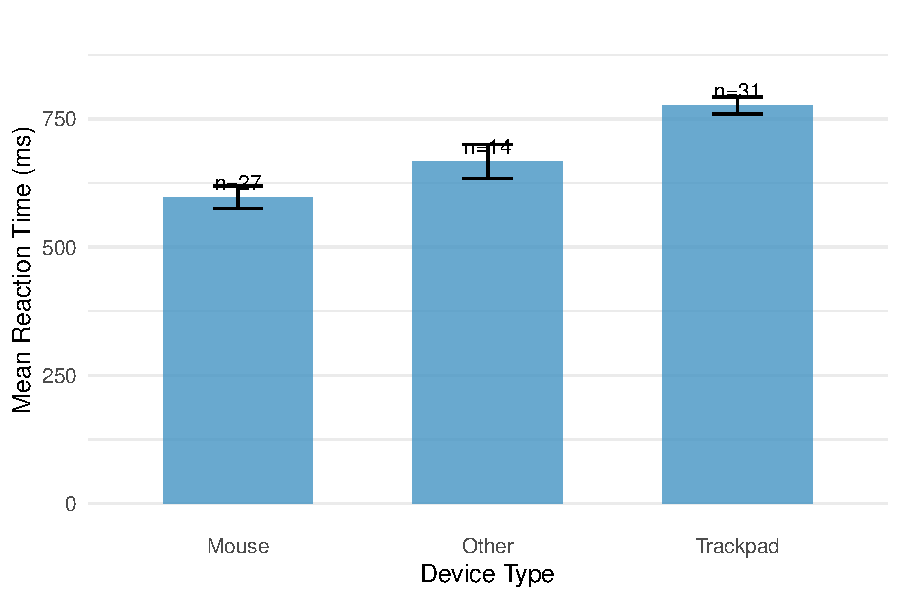
\includegraphics[width=\textwidth]{covariate_bar.pdf}
  \caption{RT by device type ($\pm$1 SE).}
\end{subfigure}
\hfill
\begin{subfigure}[t]{0.48\textwidth}
  \centering
  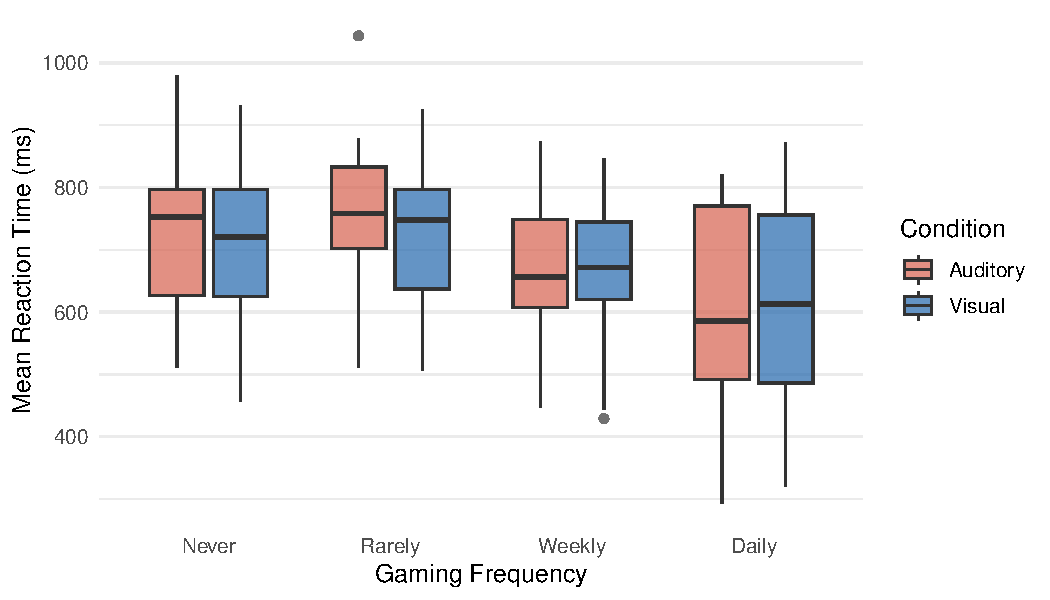
\includegraphics[width=\textwidth]{gaming_interaction.pdf}
  \caption{RT by gaming frequency and condition.}
\end{subfigure}
\caption{Covariate effects on reaction time.}
\end{figure}

\begin{figure}[H]
\centering
\begin{subfigure}[t]{0.48\textwidth}
  \centering
  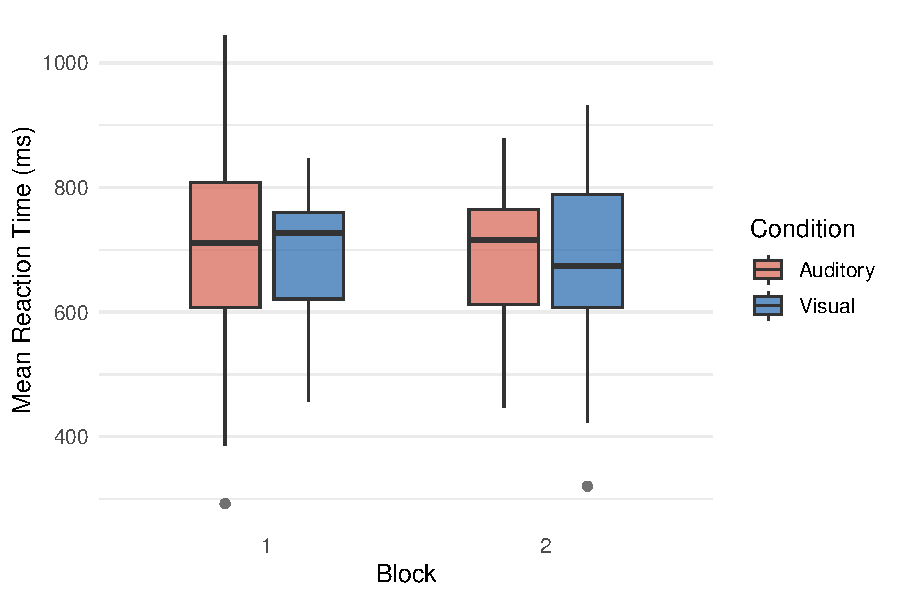
\includegraphics[width=\textwidth]{block_comparison.pdf}
  \caption{RT by block ($p = .281$, $d = 0.13$).}
\end{subfigure}
\hfill
\begin{subfigure}[t]{0.48\textwidth}
  \centering
  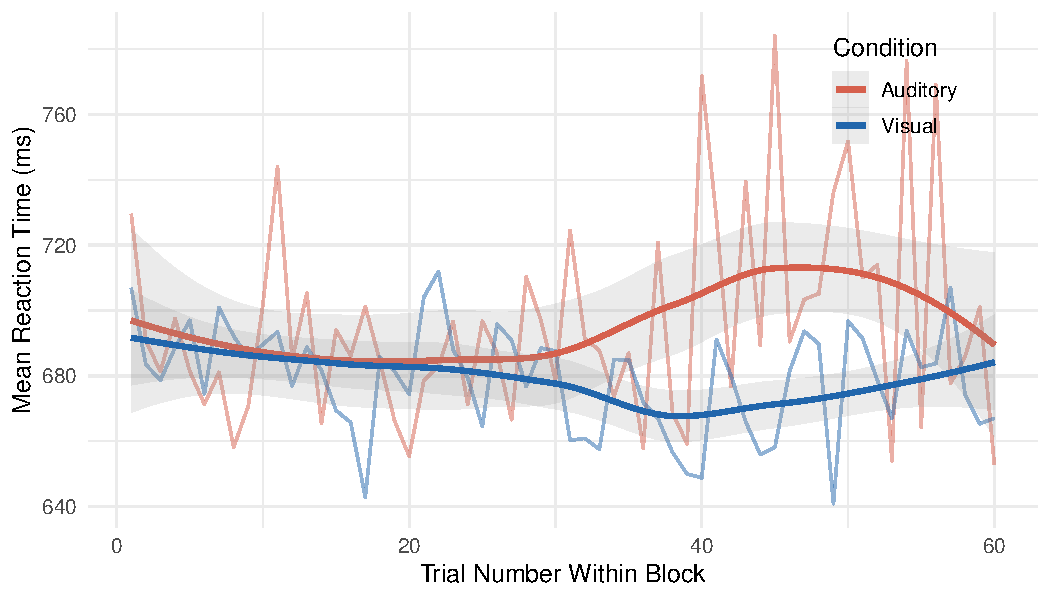
\includegraphics[width=\textwidth]{learning_curve.pdf}
  \caption{RT by trial number within block.}
\end{subfigure}
\caption{Block and learning effects.}
\end{figure}

\begin{figure}[H]
\centering
\begin{subfigure}[t]{0.48\textwidth}
  \centering
  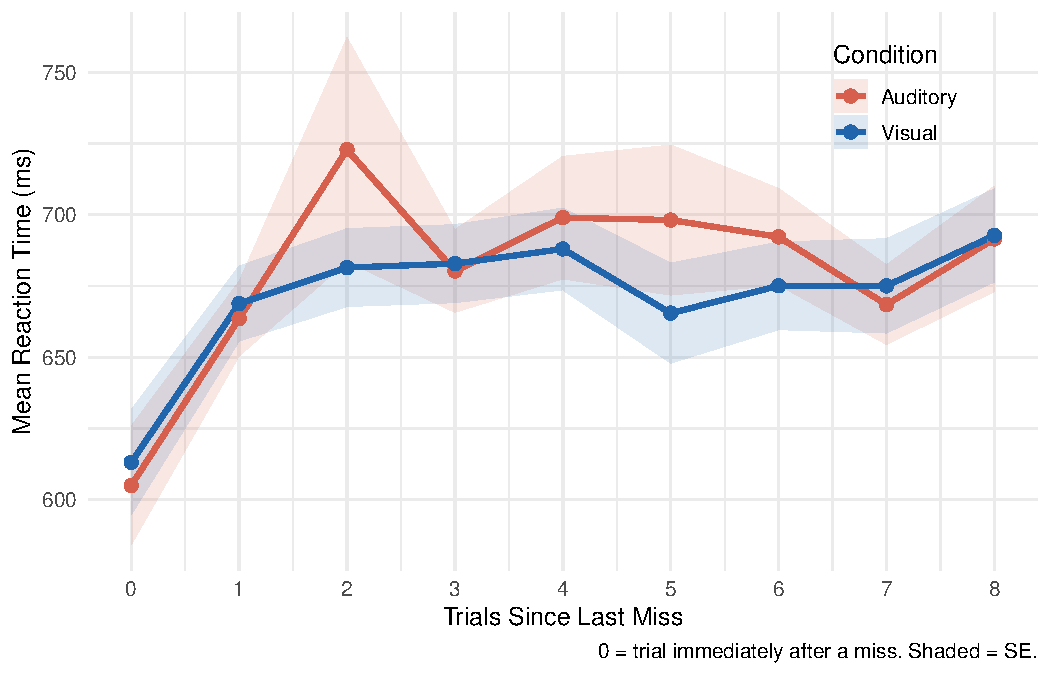
\includegraphics[width=\textwidth]{post_miss_rt.pdf}
  \caption{RT trajectory after a miss. Visual participants slow down 65.5\,ms vs.\ 17.4\,ms for auditory.}
  \label{fig:postmiss}
\end{subfigure}
\hfill
\begin{subfigure}[t]{0.48\textwidth}
  \centering
  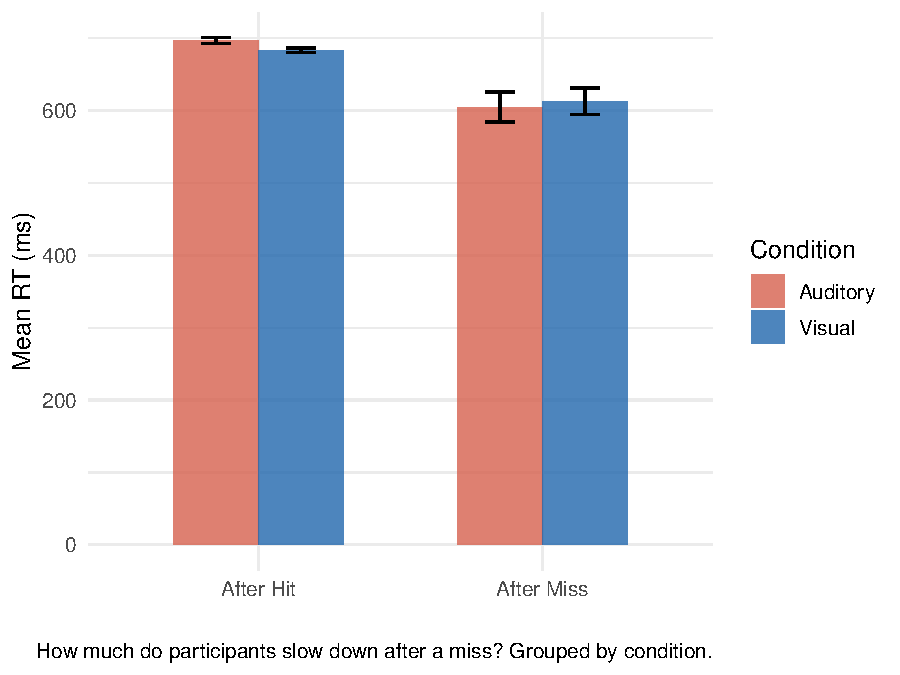
\includegraphics[width=\textwidth]{rt_after_miss_bar.pdf}
  \caption{Mean RT after hit vs.\ after miss, by condition.}
\end{subfigure}
\caption{Post-miss behavior: visual feedback makes failure more salient.}
\end{figure}

\section{Experiment Interface}

\begin{figure}[H]
\centering
\begin{subfigure}[t]{0.48\textwidth}
  \centering
  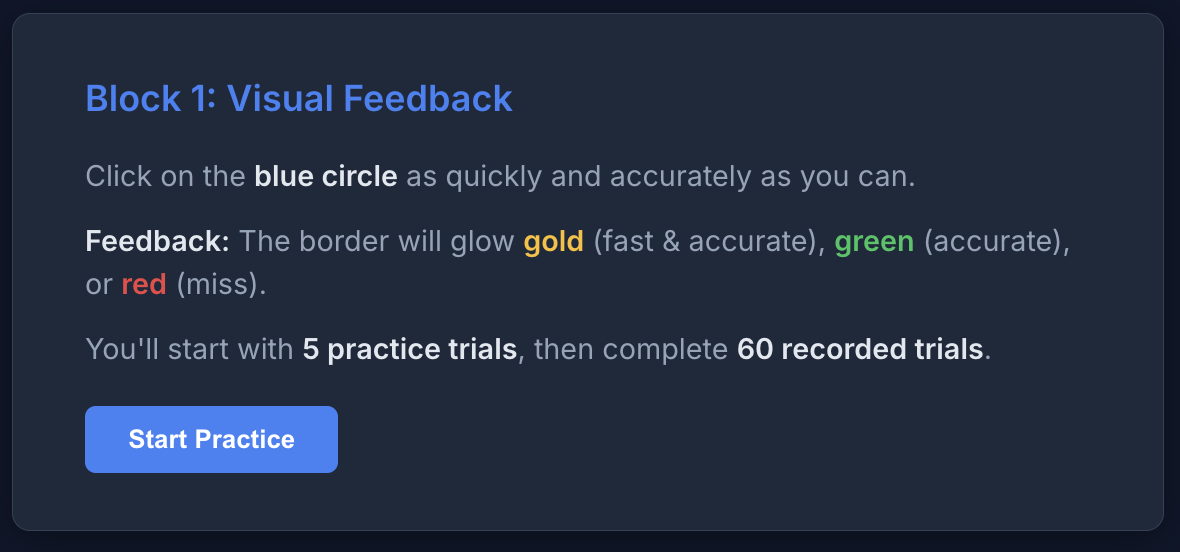
\includegraphics[width=\textwidth]{visual_information_block.png}
  \caption{Visual condition instructions.}
\end{subfigure}
\hfill
\begin{subfigure}[t]{0.48\textwidth}
  \centering
  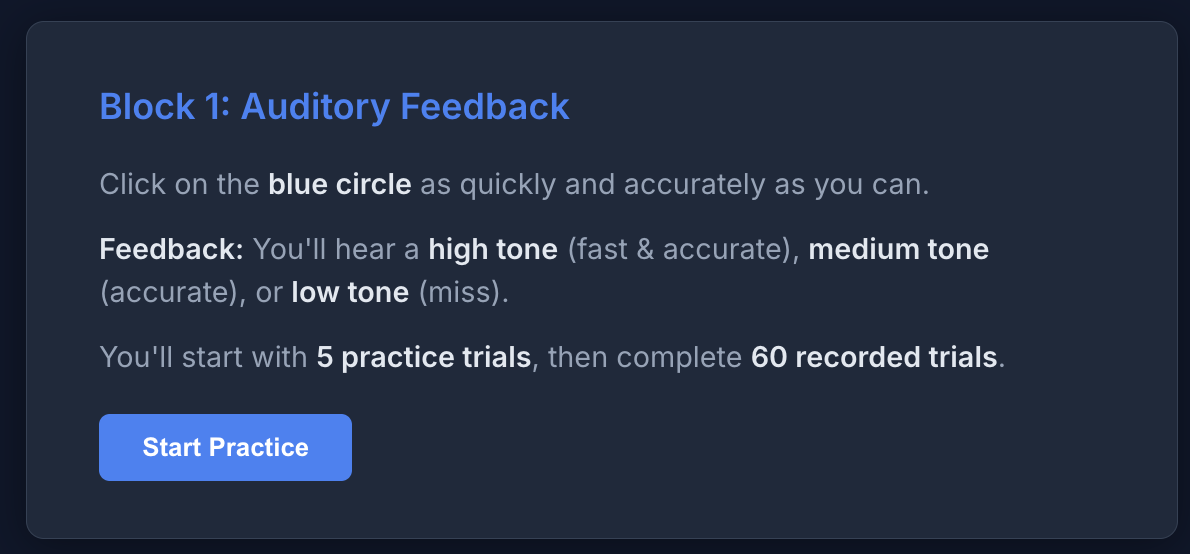
\includegraphics[width=\textwidth]{auditory_information_block.png}
  \caption{Auditory condition instructions.}
\end{subfigure}
\caption{Instruction screens. Both describe the same task; only the feedback description differs.}
\end{figure}

\begin{figure}[H]
\centering
\begin{subfigure}[t]{0.48\textwidth}
  \centering
  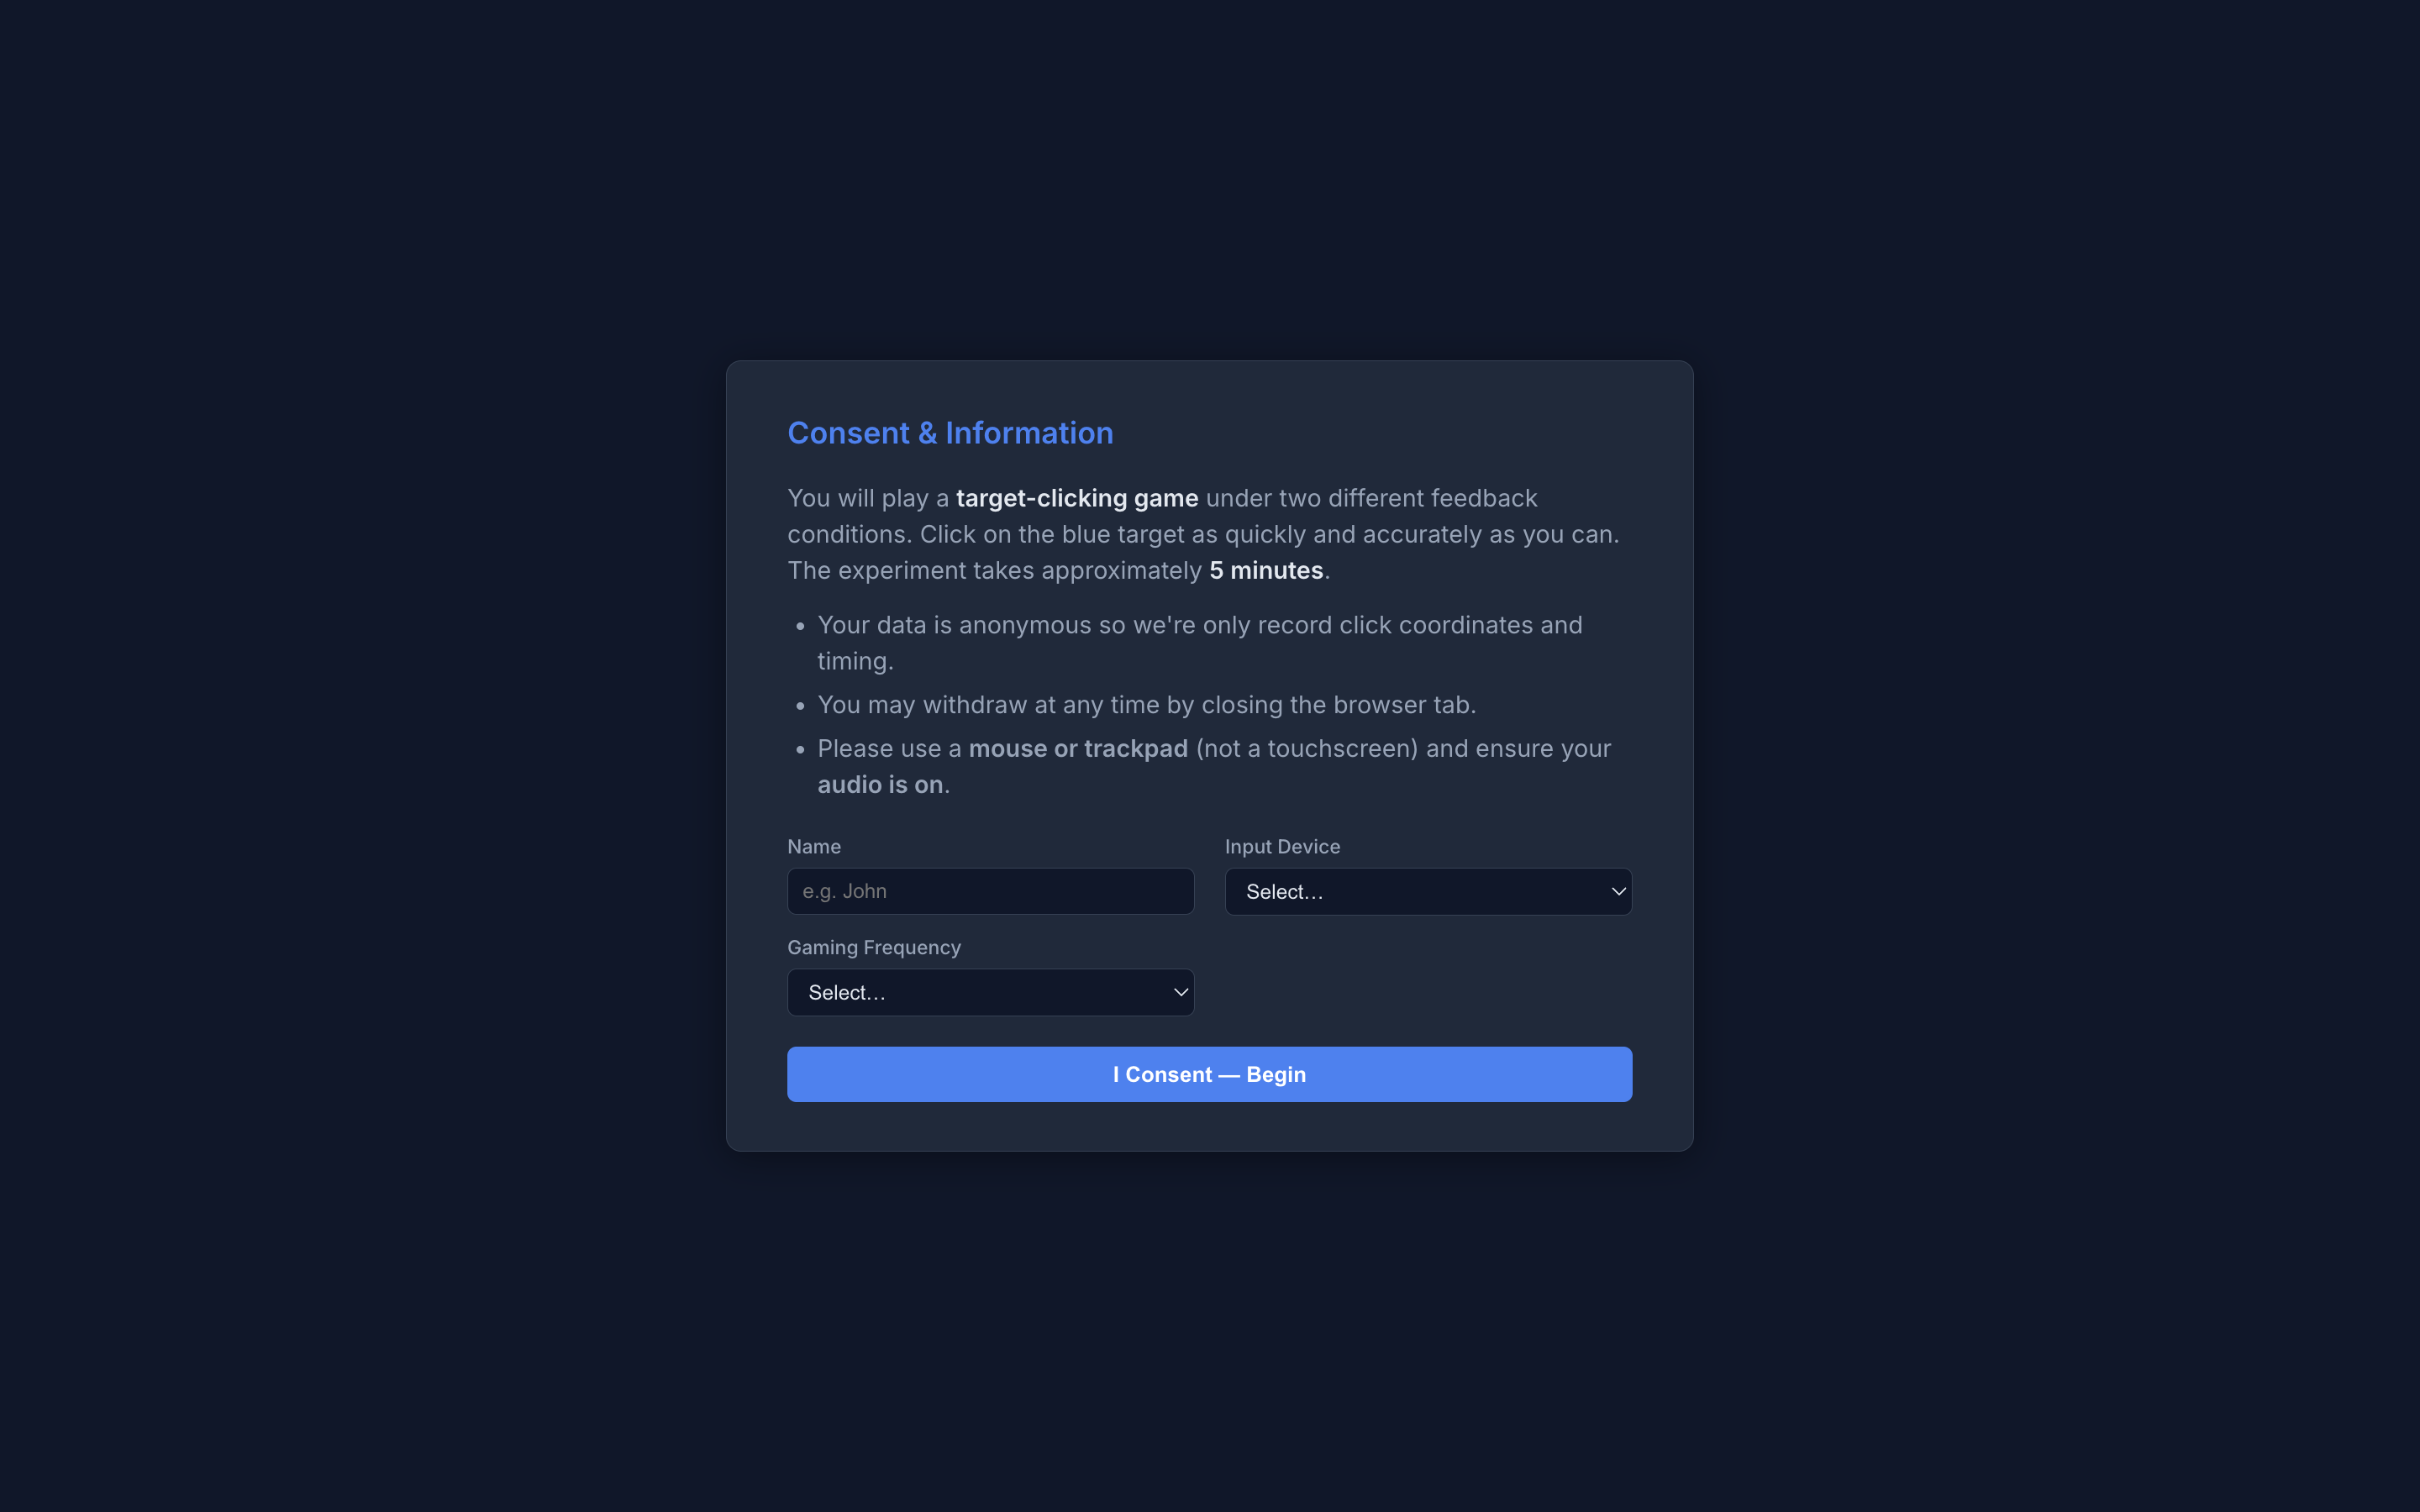
\includegraphics[width=\textwidth]{consent_screen.png}
  \caption{Consent and demographics.}
\end{subfigure}
\hfill
\begin{subfigure}[t]{0.48\textwidth}
  \centering
  
\includegraphics[width=\textwidth]{leaderboard.png}
  \caption{Leaderboard with superlatives.}
\end{subfigure}
\caption{Data collection interface and leaderboard.}
\end{figure}


\section{Additional Analyses}

\begin{figure}[H]
\centering
\begin{subfigure}[t]{0.48\textwidth}
  \centering
  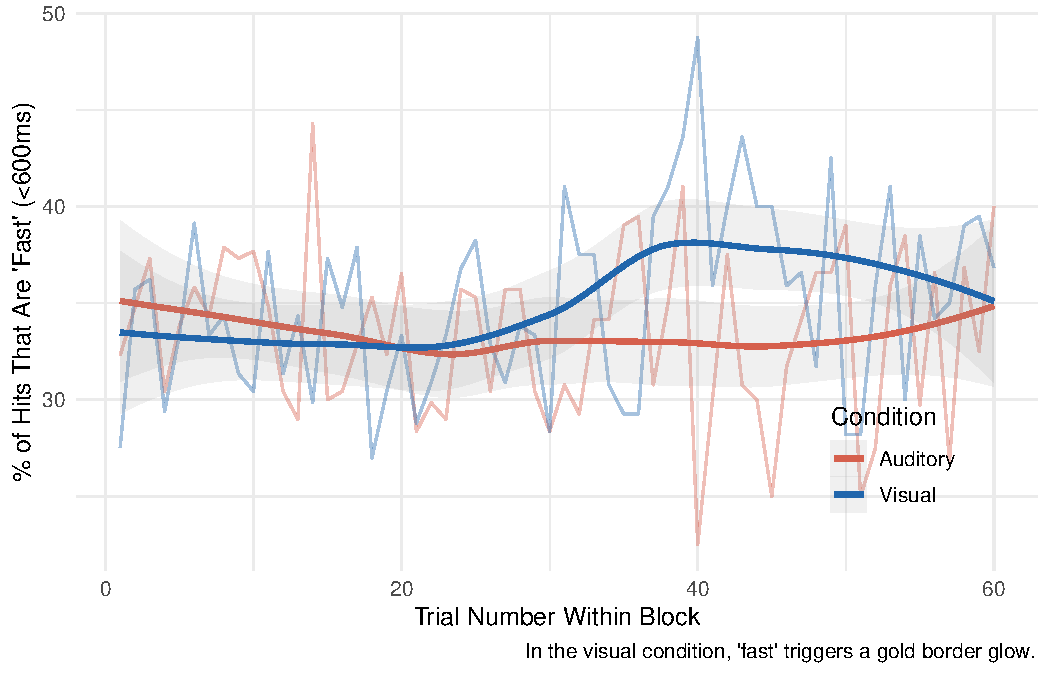
\includegraphics[width=\textwidth]{gold_chasing.pdf}
  \caption{Gold-chasing: \% of fast ($<$600\,ms) hits over trial number. Visual condition triggers gold glow for fast hits.}
\end{subfigure}
\hfill
\begin{subfigure}[t]{0.48\textwidth}
  \centering
  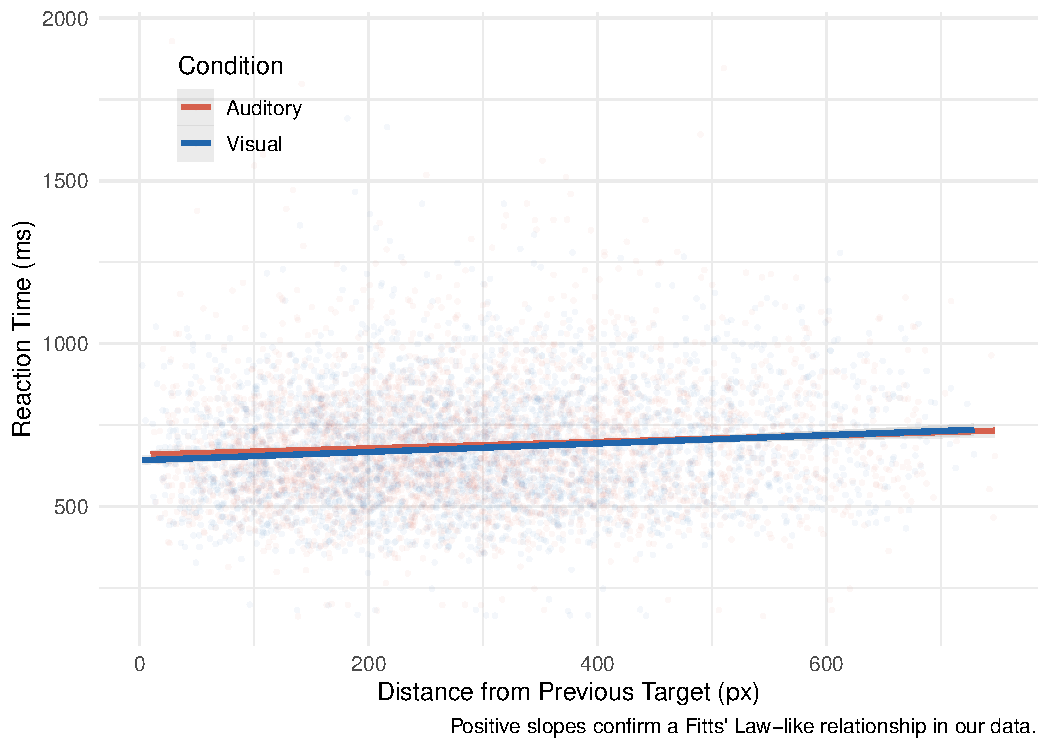
\includegraphics[width=\textwidth]{fitts_law.pdf}
  \caption{Fitts' Law: inter-target distance predicts RT ($p < .001$). Visual slope is steeper (0.13 vs 0.10\,ms/px).}
\end{subfigure}
\caption{Gold-chasing behavior and Fitts' Law relationships by condition.}
\end{figure}

\begin{figure}[H]
\centering
\begin{subfigure}[t]{0.48\textwidth}
  \centering
  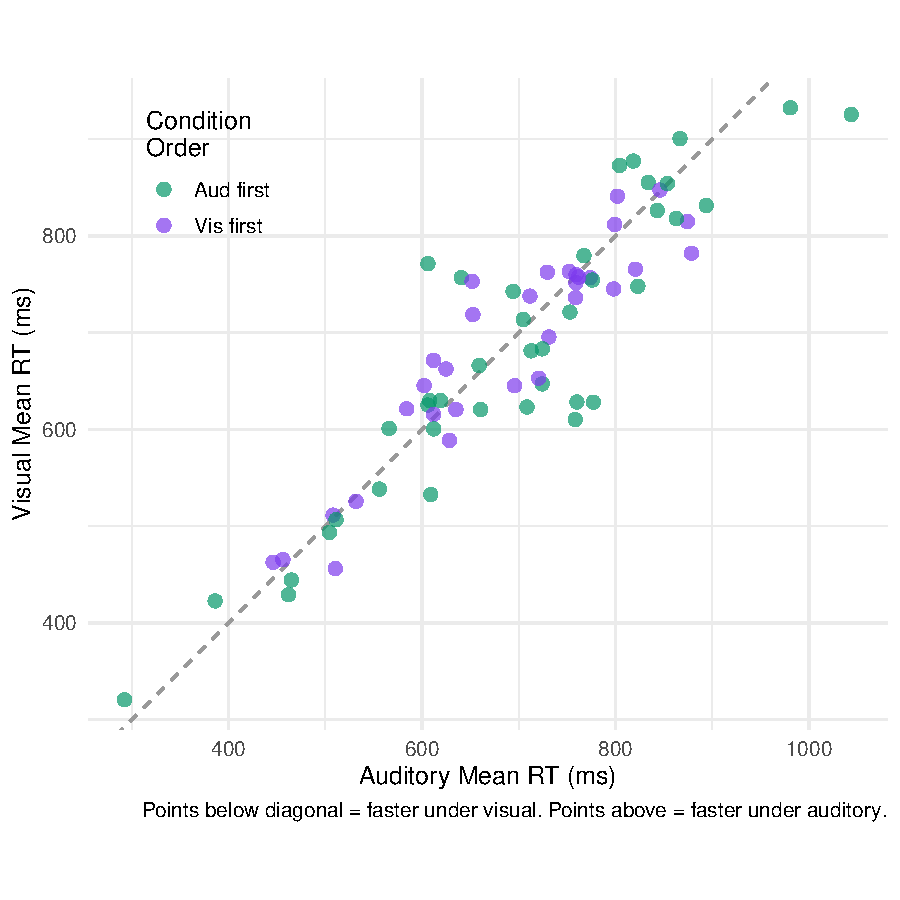
\includegraphics[width=\textwidth]{paired_scatter.pdf}
  \caption{Per-participant: visual RT vs auditory RT. Below diagonal = faster under visual.}
\end{subfigure}
\hfill
\begin{subfigure}[t]{0.48\textwidth}
  \centering
  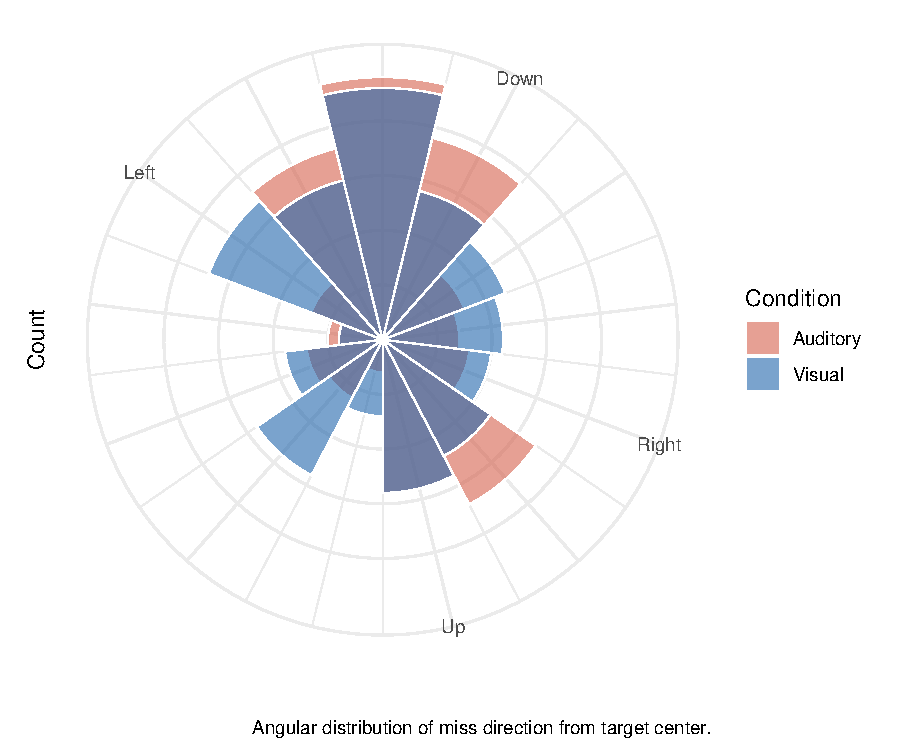
\includegraphics[width=\textwidth]{miss_direction.pdf}
  \caption{Polar histogram of miss direction from target. Shows systematic rightward and downward bias.}
\end{subfigure}
\caption{Individual differences and spatial miss patterns.}
\end{figure}

\begin{figure}[H]
\centering
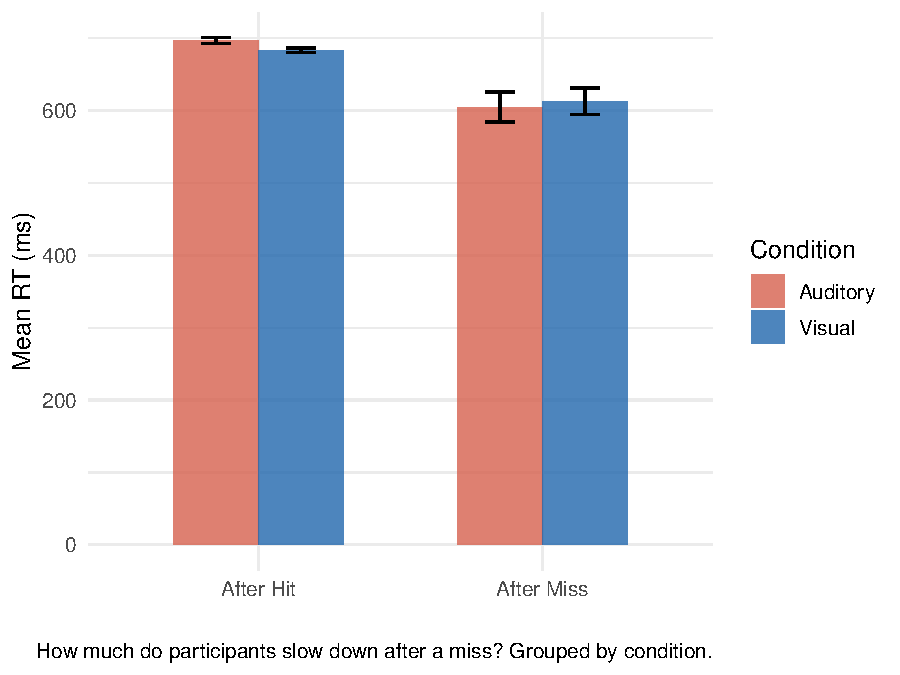
\includegraphics[width=0.65\textwidth]{rt_after_miss_bar.pdf}
\caption{Mean RT after a hit vs.\ after a miss, by condition. Visual participants slow down 65.5\,ms after a miss vs.\ 17.4\,ms for auditory, suggesting visual feedback makes failure more salient.}
\end{figure}

\section{R Code}

All analyses were conducted in R~4.5. The pipeline consists of six scripts run sequentially via \texttt{00\_run\_all.R}:

\begin{enumerate}
  \item \texttt{01\_load\_clean.R} : Load all CSVs, exclude RT outliers, filter to 60-trial participants ($N = 41$), aggregate per-participant means.
  \item \texttt{02\_descriptives.R} : Summary tables by condition, device, gaming frequency.
  \item \texttt{03\_assumptions.R} : Shapiro--Wilk tests and QQ plots.
  \item \texttt{04\_inferential.R} : Paired $t$-test (H\textsubscript{1}), Wilcoxon (H\textsubscript{2}), multiple regression with interaction (H\textsubscript{3}).
  \item \texttt{05\_plots.R} : All figures.
  \item \texttt{06\_secondary.R} : Tilt effect, order check, variance, block comparison, spatial bias.
\end{enumerate}

Full code is in the \texttt{analysis/scripts/} directory submitted alongside this report.


\section{30 vs.\ 60 Trial Comparison}
\label{app:30v60}

To justify the shift from 30 to 60 trials per block, we compared the statistical results across both cohorts. Table~\ref{tab:30v60} shows that the 30-trial participants ($N = 31$) produced no significant effects for any hypothesis, while the 60-trial participants ($N = 41$) produced significant results for all three. The 30-trial group added between-participant noise without contributing sufficient within-participant data for stable estimates.

\begin{table}[H]
\centering
\caption{Comparison of statistical results by trial count.}
\label{tab:30v60}
\begin{tabular}{lccccc}
\toprule
& \multicolumn{2}{c}{\textbf{30 trials ($N=31$)}} & \multicolumn{2}{c}{\textbf{60 trials ($N=41$)}} \\
\cmidrule(lr){2-3} \cmidrule(lr){4-5}
& Statistic & $p$ & Statistic & $p$ \\
\midrule
H\textsubscript{1}: RT & $t = 0.21$ & $.837$ & $t = -2.05$ & $.047$* \\
H\textsubscript{2}: Error & $V = 203$ & $.811$ & $V = 580$ & $.026$* \\
H\textsubscript{3}: Interaction & $\beta_3 = 0.018$ & $.163$ & $\beta_3 = -0.011$ & $<.001$*** \\
\midrule
Mean RT diff (ms) & \multicolumn{2}{c}{$+2.0$} & \multicolumn{2}{c}{$-18.5$} \\
Mean error diff (px) & \multicolumn{2}{c}{$-2.5$} & \multicolumn{2}{c}{$+1.0$} \\
\bottomrule
\end{tabular}
\end{table}

The 30-trial cohort showed essentially zero RT difference between conditions ($+0.5$\,ms) and an error difference in the \emph{wrong direction} ($-2.5$\,px). With only 30 trials per condition per participant, individual means were too noisy to detect the small within-subject effects. This motivated the design change to 60 trials, which provided sufficient statistical power ($d = 0.27$--$0.32$) to detect the feedback modality effect.


\end{document}
